\documentclass[titlepage]{ltjsreport}

% Figures
\usepackage{tikz}
\usetikzlibrary{
  cd,
  positioning,
}

% Tables
\usepackage{booktabs}

% Text
\usepackage{ascmac}   % for \itembox
\usepackage{enumitem}
\usepackage{epigraph}

% Math
\usepackage{amsmath}
\usepackage{amssymb}
\usepackage{amsthm}
\usepackage{mathrsfs}

% References
\usepackage[hidelinks]{hyperref}
\usepackage{cleveref}
\crefname{equation}{式}{式}
\usepackage{thmtools}
\declaretheoremstyle[
  thmbox=S,
]{mystyle}
\declaretheorem[
  style=mystyle,
  name=定理,
  refname={定理,定理},
  Refname={定理,定理},
  numberwithin=chapter,
]{theorem}
\declaretheorem[
  style=mystyle,
  name=定義,
  refname={定義,定義},
  Refname={定義,定義},
  numberlike=theorem,
]{definition}
\declaretheorem[
  style=mystyle,
  name=例,
  refname={例,例},
  Refname={例,例},
]{example}
\usepackage{proof}
\renewcommand{\proofname}{\textbf{証明}}

\newcommand{\cat}[1]{\mathscr{#1}}
\newcommand{\obj}[1]{\lowercase{#1}}
\newcommand{\objs}[1]{#1}
\newcommand{\mrp}[3]{{#1}:{#2}\to{#3}}
\newcommand{\mrps}[3]{#1(#2,#3)}
\newcommand{\id}[1]{\mathrm{id}_{#1}}
\newcommand{\op}[1]{{#1}^{\mathrm{op}}}
\newcommand{\set}{\mathbf{Set}}
\newcommand{\Cat}{\mathbf{Cat}}
\newcommand{\Fun}[2]{{#2}^{#1}}
\newcommand{\Comma}[2]{\left({#1}\downarrow{#2}\right)}
\newcommand{\Elem}[2]{\operatorname{\mathrm{el}}{(#2)}}
\newcommand{\Top}{\mathsf{Top}}
\newcommand{\blat}{\mathsf{BLat}}
\newcommand{\stone}{\mathsf{Stone}}
\newcommand{\interval}{\mathscr{I}}
\DeclareMathOperator{\dom}{dom}
\DeclareMathOperator{\cod}{cod}
\DeclareMathOperator{\colim}{Colim}
\DeclareMathOperator{\lan}{Lan}
\DeclareMathOperator{\ran}{Ran}
\DeclareMathOperator{\cone}{Cone}
\DeclareMathOperator{\cocone}{Cocone}
\DeclareMathOperator{\yoneda}{\textbf{よ}}%

\title{圏論ノート}
\author{大原玄嗣}

\begin{document}

\maketitle
\tableofcontents

\chapter{圏・函手・自然変換}

\section{圏}

射は,圏という世界における関係を表す矢印であり,
圏論において対象は矢印の始まりと終わりにつけられる名称に過ぎず,
対象のもつ性質は射によってのみ特徴づけられる.

\begin{definition}[圏]
  \def\a{\obj{a}}%
  \def\b{\obj{b}}%
  \def\c{\obj{c}}%
  \def\d{\obj{d}}%
  圏 (category) は,対象 (object) と射 (arrow, morphism) の集まりからなり,
  以下を満たす.
  \begin{itemize}
    \item 任意の射は,域 (domain) と余域 (codomain) と呼ばれる対象をもつ.
          対象 $\a$ を域,対象 $\b$ を余域とする射 $f$ を
          $\mrp{f}{\a}{\b}$ と表記する.
    \item 任意の射 $\mrp{f}{\a}{\b},\mrp{g}{\b}{\c}$ について,
          $f,g$ の合成 (composition) $\mrp{g\circ f}{\a}{\c}$
          が一意に存在する.
    \item 任意の射 $\mrp{f}{\a}{\b},\mrp{g}{\b}{\c},\mrp{h}{\c}{\d}$ について,
          $h\circ(g\circ f)=(h\circ g)\circ f$ が成り立つ.
    \item 任意の対象 $\b$ について恒等射 (identity)
          $\mrp{\id{\b}}{\b}{\b}$ が一意に存在し,
          任意の射 $\mrp{f}{\a}{\b},\mrp{g}{\b}{\c}$ について
          $\id{\b}\circ f=f$ かつ $g\circ\id{\b}=g$ が成り立つ.
  \end{itemize}
  また,圏 $\cat{C}$ の対象の集まりを $\objs{\cat{C}}$,
  射 $\a\to\b$ の集まりを $\mrps{\cat{C}}{\a}{\b}$ と表記する.
  \begin{center}
    \begin{tikzpicture}
      \node (A) {$\a$};
      \node [right=1cm of A] (B) {$\b$};
      \node [right=1cm of B] (C) {$\c$};
      \node [above=1.5cm of B] (catc) {$\cat{C}$};
      \draw [->] (A) to [edge label=$f$] (B);
      \draw [->] (B) to [edge label=$g$] (C);
      \draw [->, bend right] (A) to node [below] {$g\circ f$} (C);
      \draw [->, loop above] (A) to node [above] {$\id{\a}$} (A);
      \draw [->, loop above] (B) to node [above] {$\id{\b}$} (B);
      \draw [->, loop above] (C) to node [above] {$\id{\c}$} (C);
    \end{tikzpicture}
  \end{center}
\end{definition}

\begin{definition}[逆射]
  \def\a{\obj{a}}%
  \def\b{\obj{b}}%
  射 $\mrp{f}{\a}{\b}$ について以下を満たす射 $\mrp{g}{\b}{\a}$ を
  $f$ の逆射 (inverse) といい,
  $f^{-1}$ と表記する:
  \begin{equation}
    g\circ f=\id{\a}\wedge f\circ g=\id{\b}.
  \end{equation}
\end{definition}

\begin{theorem}[逆射の一意性]
  任意の射について,逆射は高々1つである.
\end{theorem}

\begin{proof}
  \def\a{\obj{a}}%
  \def\b{\obj{b}}%
  射 $\mrp{f}{\a}{\b}$ の相異なる逆射 $\mrp{g,h}{\b}{\a}$ が存在すると仮定する.
  \begin{equation*}
    g=g\circ\id{\b}=g\circ(f\circ h)=(g\circ f)\circ h=\id{\a}\circ h=h.
  \end{equation*}
  これは仮定に矛盾し,定理は示された.
\end{proof}

\begin{definition}[同型射]
  射 $f$ について逆射 $f^{-1}$ が存在するとき,
  $f$ は同型射 (isomorphism) であるという.
\end{definition}

対象は性質をもたないため,
対象どうしの「本質的な等しさ」なるものも射によって定められる.

\begin{definition}[同型]
  \def\a{\obj{a}}%
  \def\b{\obj{b}}%
  圏 $\cat{C}$ の対象 $\a,\b$ について同型射 $\a\to\b$ が存在するとき,
  $\a$ と $\b$ は同型 (isomorphic) であるといい,$\a\simeq\b$ と表記する.
\end{definition}

\subsection{圏の大きさ}

\begin{definition}[局所小圏]
  \def\C{\cat{C}}%
  \def\a{\obj{a}}%
  \def\b{\obj{b}}%
  圏 $\C$ の任意の対象 $\a,\b\in\C$ について
  $\mrps{\C}{\a}{\b}$ が小さい集合 (\cref{def:small-set}) であるとき,
  $\C$ を局所小圏 (locally small category) という.
\end{definition}

\subsection{さまざまな圏}

\begin{definition}[離散圏]
  任意の射が恒等射である圏を離散圏 (discrete category) といい,
  対象の集まりが有限である場合は対象の数を用いて
  $\mathbf{0},\mathbf{1},\mathbf{2},\ldots$ と表記する.
  特に $\mathbf{0}$ を空圏 (empty category) といい,
  $\mathbf{1}$ を終圏 (terminal category) または
  自明な圏 (trivial category) という.
\end{definition}

\begin{definition}[区間圏]\label{def:interval-category}
  2 つの対象 $0,1$ および唯一の非自明な射 $0\to1$ からなる圏を
  区間圏 (interval category) といい,$\interval$ と表記する.
\end{definition}

前述のとおり,圏論では対象そのものが既に何らかの性質を備えているとは考えない.
むしろ対象の「性質」とは他の対象との関係性によって初めて問題にできるものだ.

素朴な集合論においては,
まず集合が要素をもち,それらの対応づけとして集合間の写像が定義される.
圏論はその逆をいく.「集合」という何かの間に写像を定めてしまい,
それによって初めて集合の要素を定義する.

\begin{definition}[集合圏]
  集合圏は,任意の集合を対象とし,それらの間の任意の写像を射とする圏である.
\end{definition}

\section{函手}

2つの世界 (圏) を比較したときに,世界を構成する要素は全く違っていても,
それらの関係性に着目するとなんとなく似ている気がしてくることがある.
函手はそのようなアナロジーを表現する矢印である.
\begin{definition}[函手]\label{def:functor}
  \def\C{\cat{C}}%
  \def\D{\cat{D}}%
  \def\x{\obj{x}}%
  \def\y{\obj{y}}%
  \def\z{\obj{z}}%
  圏 $\C,\D$ について,
  対象 $\x\in\objs{\C}$ を対象 $F(\x)\in\objs{\D}$ に写し,
  射 $f\in\mrps{\C}{\x}{\y}$ を射 $F(f)\in\mrps{\D}{F(\x)}{F(\y)}$ に写す
  マップ $F$ が以下の条件を満たすとき,
  $F$ を $\C$ から $\D$ への函手 (functor) といい,
  $\mrp{F}{\C}{\D}$ と表記する.
  \begin{align}
    \forall f\in\mrps{\C}{\x}{\y}\ \forall g\in\mrps{\C}{\y}{\z};
     & \ F(g\circ f)=F(g)\circ F(f), \\
    \forall\x\in\objs{\C};
     & \ F(\id{\x})=\id{F(\x)}.
  \end{align}
  \begin{center}
    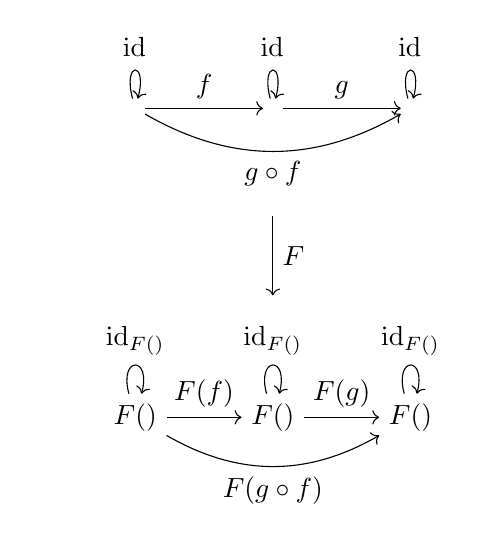
\begin{tikzpicture}
      \node (catc) {$\C$};
      \node [right=1.0cm of catc] (A) {$\x$};
      \node [right=1.5cm of A] (B) {$\y$};
      \node [right=1.5cm of B] (C) {$\z$};
      \node [below=3.5cm of catc] (catd) {$\D$};
      \node [below=3.5cm of A] (FA) {$F(\x)$};
      \node [below=3.5cm of B] (FB) {$F(\y)$};
      \node [below=3.5cm of C] (FC) {$F(\z)$};
      \draw [->] (A) to node [above] {$f$} (B);
      \draw [->] (B) to node [above] {$g$} (C);
      \draw [->, bend right] (A) to node [below] {$g\circ f$} (C);
      \draw [->, loop above] (A) to node [above] {$\id{\x}$} (A);
      \draw [->, loop above] (B) to node [above] {$\id{\y}$} (B);
      \draw [->, loop above] (C) to node [above] {$\id{\z}$} (C);
      \draw [->] (FA) to node [above] {$F(f)$} (FB);
      \draw [->] (FB) to node [above] {$F(g)$} (FC);
      \draw [->, bend right] (FA) to node [below] {$F(g\circ f)$} (FC);
      \draw [->, loop above] (FA) to node [above] {$\id{F(\x)}$} (FA);
      \draw [->, loop above] (FB) to node [above] {$\id{F(\y)}$} (FB);
      \draw [->, loop above] (FC) to node [above] {$\id{F(\z)}$} (FC);
      \node [below=1cm of B] (from) {};
      \node [above=1cm of FB] (to) {};
      \draw [->] (from) to node [right] {$F$} (to);
    \end{tikzpicture}
  \end{center}
\end{definition}

\begin{shadebox}
  \def\C{\cat{C}}%
  \def\D{\cat{D}}%
  \def\c{\obj{c}}%
  \def\d{\obj{d}}%
  \def\e{e}%
  \def\F{F}%
  \cref{def:functor} では函手に (i) 合成の保存と (ii) 恒等射の保存の二条件が
  要求されている.
  ここで, (i) が (ii) を含意するのではないか,この定義は冗長ではないかと
  疑問に思われたかもしれないが,一般に (i) は (ii) を含意しない.
  以下のような場合を考える.
  \begin{itemize}
    \item 圏 $\C$ は対象 $\c$ と恒等射 $\id{\c}$ のみからなる.
    \item 圏 $\D$ は対象 $\d$ と恒等射 $\id{\d}$ ,射 $\mrp{e}{\d}{\d}$
          のみからなり,$\e=\e\circ\e$ である.
  \end{itemize}
  ここで $\F(\id{\c})=\e$ であるような対応 $\F$ は
  (i) を満たすが (ii) を満たさない.
\end{shadebox}

\begin{definition}[充満,忠実,充満忠実]\label{def:full-faithful}
  \def\C{\cat{C}}%
  \def\D{\cat{D}}%
  \def\x{\obj{x}}%
  \def\y{\obj{y}}%
  函手 $\mrp{F}{\C}{\D}$ および任意の対象 $\x,\y\in\objs{\C}$ に対して,
  射についての対応 $\mrps{\C}{\x}{\y}\to\mrps{\D}{F(\x)}{F(\y)}$ が
  \begin{itemize}
    \item 全射であるとき $F$ は充満 (full) であるといい,
    \item 単射であるとき $F$ は忠実 (faithful) であるという.
  \end{itemize}
  また $F$ が充満かつ忠実であるとき,
  $F$ は充満忠実 (full and faithful, fully faithful) であるという.
\end{definition}

{

\subsection{圏の圏 $\Cat$}

\def\C{\cat{C}}%
\def\D{\cat{D}}%
\def\E{\cat{E}}%
\def\F{F}%
\def\G{G}%
\def\a{\obj{a}}%
\def\b{\obj{b}}%
\def\c{\obj{c}}%
\def\f{f}%
\def\g{g}%

\begin{definition}[函手の合成]
  函手 $\mrp{\F}{\C}{\D},\mrp{\G}{\D}{\E}$ について,
  以下のように定められるマップを $\F$ と $\G$ の合成といい,
  $\G\circ\F$ と表記する.
  \begin{align}
    \C\ni\a                & \mapsto\G(\F(\a))\in\E,                  \\
    \mrps{\C}{\a}{\b}\ni\f & \mapsto\mrps{\E}{\G(\F(a))}{\G(\F(\b))}.
  \end{align}
\end{definition}

\begin{theorem}
  任意の函手 $\mrp{\F}{\C}{\D},\mrp{\G}{\D}{\E}$ について,
  合成 $\G\circ\F$ は $\C$ から $\E$ への函手である.
\end{theorem}

\begin{proof}
  (i) $\G\circ\F$ が合成を保存することを示す.
  $\C$ の任意の射 $\mrp{\f}{\a}{\b},\mrp{\g}{\b}{\c}$ について
  \begin{align*}
    (\G\circ\F)(\g\circ\f)
     & =\G(\F(\g\circ\f))                    \\
     & =\G(\F(\g)\circ\F(\f))                \\
     & =\G(\F(\g))\circ\G(\F(\f))            \\
     & =(\G\circ\F)(\g)\circ(\G\circ\F)(\f).
  \end{align*}

  (ii) $\G\circ\F$ が恒等射を保存することを示す.
  $\C$ の任意の対象 $\a$ について
  \begin{align*}
    (\G\circ\F)(\id{\a})
     & =\G(\F(\id{\a}))       \\
     & =\G(\id{\F(\a)})       \\
     & =\id{\G(\F(\a))}       \\
     & =\id{(\G\circ\F)(\a)}.
  \end{align*}
\end{proof}

}

\section{自然変換}

2つの世界 (圏) について異なるアナロジーを考えることもできる.
すると,異なるアナロジーの間にも何らかのアナロジーが見えてくることがある.
この高次のアナロジーが自然変換である.

\begin{definition}[自然変換]
  \def\x{\obj{x}}%
  \def\y{\obj{y}}%
  2つの函手 $F:\cat{C}\to\cat{D},G:\cat{C}\to\cat{D}$ について,
  $\cat{C}$ の対象 $\x$ を $\cat{D}$ の射 $t_{\x}:F(\x)\to G(\x)$ に対応づける
  写像 $t$ が
  \begin{equation}
    \forall\x,\y\ \forall\mrp{f}{\x}{\y}\ G(f)\circ t_{\x}=t_{\y}\circ F(f)
  \end{equation}
  を満たすとき,$t$ を自然変換 (natural transformation) といい,
  $\mrp{t}{F}{G}$ と表記する.
  \begin{center}
    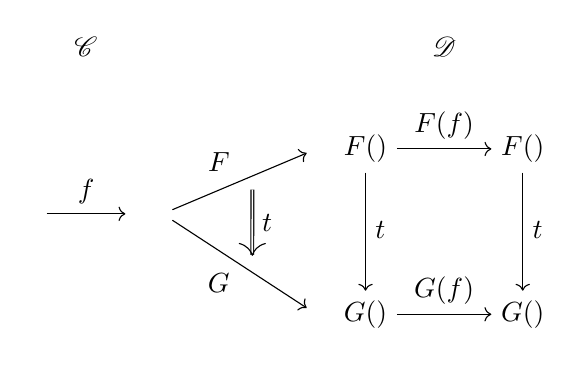
\begin{tikzpicture}
      \node (catc) {$\cat{C}$};
      \node [below left=2cm and 0.5cm of catc.center] (A) {$\x$};
      \node [right=1.0cm of A] (B) {$\y$};
      \node [right=4.0cm of catc] (catd) {$\cat{D}$};
      \node [below left=1cm and 0.6cm of catd.center] (FA) {$F(\x)$};
      \node [right=1.2cm of FA] (FB) {$F(\y)$};
      \node [below=1.8cm of FA.center] (GA) {$G(\y)$};
      \node [below=1.8cm of FB.center] (GB) {$G(\y)$};
      \draw [->] (A) to node [above] {$f$} (B);
      \draw [->] (FA) to node [above] {$F(f)$} (FB);
      \draw [->] (GA) to node [above] {$G(f)$} (GB);
      \draw [->] (FA) to node [right] {$t_{\x}$} (GA);
      \draw [->] (FB) to node [right] {$t_{\y}$} (GB);
      \node [right=0.1cm of B] (from) {};
      \node [left=0.1cm of FA] (fto) {};
      \draw [->] (from) to node [above left] (F) {$F$} (fto);
      \node [left=0.1cm of GA] (gto) {};
      \draw [->] (from) to node [below left] (G) {$G$} (gto);
      \node [below right=0.1cm and 0.3cm of F.center] (tfrom) {};
      \node [above right=0.1cm and 0.3cm of G.center] (tto) {};
      \draw [->,double] (tfrom) to node [right] {$t$} (tto);
    \end{tikzpicture}
  \end{center}
\end{definition}

\begin{definition}[垂直合成]
  \def\C{\cat{C}}%
  \def\D{\cat{D}}%
  \def\F{F}%
  \def\G{G}%
  \def\h{H}%
  \def\c{\obj{c}}%
  函手 $\mrp{\F,\G,\h}{\C}{\D}$ および自然変換
  $\mrp{\theta}{\F}{\G},\mrp{\sigma}{\G}{\h}$
  について対象 $\c\in\C$ を $\D$ の射
  $\mrp{{\sigma}_{\c}\circ{\theta}_{\c}}{\F(\c)}{\h(\c)}$
  に写すマップを
  $\theta$ と $\sigma$ の垂直合成 (vertical composition) といい,
  $\sigma\circ\theta$ と表記する.
\end{definition}

\chapter{極限}

\section{普遍射}

 {
  \def\C{\cat{C}}%
  \def\D{\cat{D}}%
  \def\c{\obj{c}}%
  \def\d{\obj{d}}%
  \def\r{\obj{r}}%
  \def\S{S}%
  \def\f{f}%
  \def\g{f'}%
  \def\unia{v}%
  \def\unib{u}%

  \begin{definition}[普遍射-1]
    函手 $\mrp{S}{\D}{\C}$ と対象 $\c\in\objs{\C}$ について,
    対象 $\r\in\objs{\D}$ と射 $\mrp{\unia}{\S(\r)}{\c}$ の組 $(\r,\unia)$ が
    \begin{equation}
      \forall\d\in\objs{\D}\ \forall\f\in\mrps{\C}{\S(\d)}{\c}
      \ \exists!\g\in\mrps{\D}{\d}{\r};\ \f=\unia\circ\S(\g)
    \end{equation}
    を満たすとき,$(\r,\unia)$ を $\S$ から $\c$ への普遍射 (universal arrow) という.
    \begin{center}
      \begin{tikzcd}[column sep=0.8cm]
        &\C
        &\D\arrow{l}[swap]{\S} \\
        & \S(\d)\arrow[dashed]{d}{\S(\g)}\arrow{ld}[swap]{\f}
        & \d\arrow[dashed]{d}{\g} \\
        \c & \S(\r)\arrow{l}{\unia} & \r
      \end{tikzcd}
    \end{center}
  \end{definition}

  \begin{definition}[普遍射-2]
    函手 $\mrp{\S}{\D}{\C}$ と対象 $\c\in\objs{\C}$ について,
    対象 $\r\in\objs{\D}$ と射 $\mrp{\unib}{\c}{\S(\r)}$ の組 $(\r,\unib)$ が
    \begin{equation}
      \forall\d\in\objs{\D}\ \forall\f\in\mrps{\C}{\c}{\S(\d)}
      \ \exists!\g\in\mrps{\D}{\r}{\d};\ \f=\S(\g)\circ\unib
    \end{equation}
    を満たすとき,$(\r,u)$ を $\c$ から $S$ への普遍射という.
    \begin{center}
      \begin{tikzcd}[column sep=0.8cm]
        &\C
        &\D\arrow{l}[swap]{\S} \\
        \c\arrow{r}{\unib}\arrow{rd}{\f}
        & \S(\r)\arrow[dashed]{d}{\S(\g)}
        & r\arrow[dashed]{d}{\g}\\
        & \S(\d) & \d
      \end{tikzcd}
    \end{center}
  \end{definition}
 }

\section{極限と余極限}

\begin{definition}[終対象]
  圏 $\cat{C}$ および対象 $\obj{t}\in\objs{\cat{C}}$ が
  \begin{equation}
    \forall\obj{x}\in\objs{\cat{C}};\ |\mrps{\cat{C}}{\obj{x}}{\obj{t}}|=1
  \end{equation}
  を満たすとき,
  $\obj{t}$ を $\cat{C}$ の終対象 (terminal object) という.
\end{definition}

\begin{definition}[始対象]
  圏 $\cat{C}$ および対象 $\obj{i}\in\objs{\cat{C}}$ が
  \begin{equation}
    \forall\obj{x}\in\objs{\cat{C}};\ |\mrps{\cat{C}}{\obj{i}}{\obj{x}}|=1
  \end{equation}
  を満たすとき,
  $\obj{i}$ を $\cat{C}$ の始対象 (initial object) という.
\end{definition}

\begin{center}
  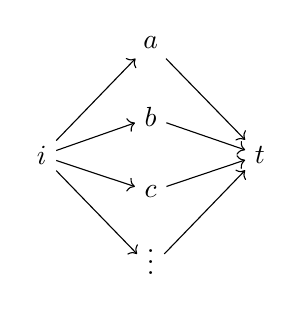
\begin{tikzpicture}
    \node (A) {$\obj{a}$};
    \node [below=0.5cm of A] (B) {$\obj{b}$};
    \node [below=0.5cm of B] (C) {$\obj{c}$};
    \node [below=0.2cm of C] (D) {$\vdots$};
    \node [below left =0.0cm and 1.0cm of B] (I) {$\obj{i}$};
    \node [below right=0.0cm and 1.0cm of B] (T) {$\obj{t}$};
    \draw [->] (I) to (A);
    \draw [->] (I) to (B);
    \draw [->] (I) to (C);
    \draw [->] (I) to (D.west);
    \draw [->] (A) to (T);
    \draw [->] (B) to (T);
    \draw [->] (C) to (T);
    \draw [->] (D.east) to (T);
  \end{tikzpicture}
\end{center}

\begin{definition}[定函手]
  圏 $\cat{C},\cat{D}$ および対象 $\obj{d}\in\objs{\cat{D}}$ について,
  $\cat{C}$ の任意の対象を $\obj{d}$ に写し,
  $\cat{C}$ の任意の射を $\id{\obj{d}}$ に写す函手を
  $\obj{d}$ の定函手 (constant functor) という.
\end{definition}

\begin{definition}[対角函手]
  圏 $\cat{C},\cat{D}$ について,
  任意の対象 $\obj{d}\in\objs{\cat{D}}$ を $\obj{d}$ の定函手に写す函手
  $\mrp{\Delta}{\cat{D}}{\cat{D}^{\cat{C}}}$ を対角函手 (diagonal functor) という.
  ただし $\Delta$ は射 $f\in\mrps{\cat{D}}{a}{b}$ を,
  任意のコンポーネントが $f$ であるような自然変換
  $\mrp{\Delta(f)}{\Delta(a)}{\Delta(b)}$ に写す.
\end{definition}

\begin{definition}[錐]
  圏 $\cat{C},\cat{D}$ および函手 $\mrp{F}{\cat{C}}{\cat{D}}$ について,
  対象 $\obj{d}\in\objs{\cat{D}}$ および自然変換 $\mrp{\psi}{\id{\obj{d}}}{F}$
  の組 $(\obj{d},\psi)$ を $F$ への錐 (cone) という.
\end{definition}

\begin{definition}[余錐]
  圏 $\cat{C},\cat{D}$ および函手 $\mrp{F}{\cat{C}}{\cat{D}}$ について,
  対象 $\obj{d}\in\objs{\cat{D}}$ および自然変換 $\mrp{\phi}{F}{\id{\obj{d}}}$
  の組 $(\obj{d},\phi)$ を $F$ からの余錐 (cocone) という.
\end{definition}

\begin{definition}[錐の圏]
  函手 $F$ への錐を対象とする圏を錐の圏といい,$\cone(F)$ と表記する.
  ただし射 $u\in\mrps{\cone(F)}{(\obj{d},\psi)}{(\obj{d'},\psi')}$ は
  以下の図式を可換にする自然変換 $\id{\obj{d}}\to\id{\obj{d'}}$ である.
  \begin{center}
    \begin{tikzcd}
      \id{d}\arrow{r}{u}\arrow{d}[swap]{\psi}
      & \id{d'}\arrow{d}{\psi'} \\
      F\arrow[equal]{r}[swap]{\id{F}}
      & F
    \end{tikzcd}
  \end{center}
\end{definition}

\begin{definition}[余錐の圏]
  函手 $F$ からの余錐を対象とする圏を余錐の圏といい,$\cocone(F)$ と表記する.
  ただし射 $u\in\mrps{\cocone(F)}{(d,\phi)}{(d',\phi')}$ は
  以下の図式を可換にする自然変換 $\id{d}\to\id{d'}$ である.
  \begin{center}
    \begin{tikzcd}
      \id{d}\arrow{r}{u}
      & \id{d'} \\
      F\arrow[equal]{r}[swap]{\id{F}}\arrow{u}{\phi}
      & F\arrow{u}[swap]{\phi'}
    \end{tikzcd}
  \end{center}
\end{definition}

\begin{definition}[極限]
  $\cone(F)$ の終対象 $(\obj{t},\pi)$ を $F$ の極限 (limit) という.
  このとき $\obj{t}$ を $F$ の極限対象 (limit object) といい,
  $\obj{t}=\lim(F)$ と表記する.
\end{definition}

\begin{definition}[余極限]
  $\cocone(F)$ の始対象 $(\obj{i},\iota)$ を $F$ の余極限 (colimit) といい,
  このとき $\obj{i}$ を $F$ の余極限対象 (colimit object) といい,
  $\obj{i}=\colim(F)$ と表記する.
\end{definition}

\section{さまざまな極限}

前節では非常に抽象的な形で極限と余極限を定義した.
本節ではさまざまな図式の極限と余極限を紹介し,
それらが具体的な圏においてどのような対象に対応するのかをみていく.

\subsection{終対象と始対象}

(余) 極限の定義に用いた終対象と始対象は,
実はそれぞれ最も単純な極限と余極限として記述できる.
\begin{theorem}[極限としての終対象]
  任意の圏 $\cat{C}$ および空圏 $\cat{J}$ について,
  自明な図式 $\cat{J}\to\cat{C}$ の極限は
  $\cat{C}$ の終対象に同型である.
\end{theorem}
\begin{theorem}[余極限としての始対象]
  任意の圏 $\cat{C}$ および空圏 $\cat{J}$ について,
  自明な図式 $\cat{J}\to\cat{C}$ の余極限は
  $\cat{C}$ の始対象に同型である.
\end{theorem}
終対象や始対象の具体的な例をみてみよう.
例えば集合圏 $\set$ における終対象と始対象は,それぞれ一点集合と空集合に対応する.
一点集合 $1=\{\cdot\}$ が終対象であることは,任意の集合 $S$ について,
$S$ から $1$ への写像が $S$ の全ての要素を集合 $1$ の唯一の要素に写す写像ただひとつであることからわかる.
空集合 $\emptyset$ が始対象であることについては,
やや無理があるかもしれないが,任意の集合 $S$ について
何もしない写像 $\emptyset\to S$ がただひとつ存在するのだと考えてほしい.

\subsection{積と余積}

\begin{definition}[積]
  離散圏 $\cat{J}=\{1,2\}$ について,
  函手 $F:\cat{J}\to\cat{C}$ の極限を積 (product) といい,
  $F(1)=A,F(2)=B$ のとき $A\times B$ と表記する.
  \begin{center}
    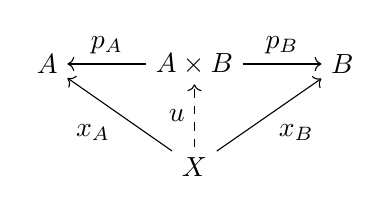
\begin{tikzpicture}
      \node (A) {$A$};
      \node [right=1.0cm of A] (P) {$A\times B$};
      \node [right=1.0cm of P] (B) {$B$};
      \node [below=0.8cm of P] (X) {$X$};
      \draw [->] (P) to node [above] {$p_A$} (A);
      \draw [->] (P) to node [above] {$p_B$} (B);
      \draw [->, dashed] (X) to node [left] {$u$} (P);
      \draw [->] (X) to node [below left] {$x_A$} (A);
      \draw [->] (X) to node [below right] {$x_B$} (B);
    \end{tikzpicture}
  \end{center}
\end{definition}

\begin{definition}[余積]
  離散圏 $\cat{J}=\{1,2\}$ について,
  函手 $F:\cat{J}\to\cat{C}$ の余極限を余積 (coproduct) といい,
  $F(1)=A,F(2)=B$ のとき $A+B$ と表記する.
  \begin{center}
    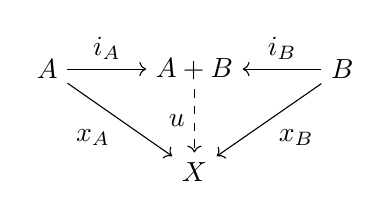
\begin{tikzpicture}
      \node (A) {$A$};
      \node [right=1.0cm of A] (Q) {$A+B$};
      \node [right=1.0cm of Q] (B) {$B$};
      \node [below=0.8cm of Q] (X) {$X$};
      \draw [->] (A) to node [above] {$i_A$} (Q);
      \draw [->] (B) to node [above] {$i_B$} (Q);
      \draw [->, dashed] (Q) to node [left] {$u$} (X);
      \draw [->] (A) to node [below left] {$x_A$} (X);
      \draw [->] (B) to node [below right] {$x_B$} (X);
    \end{tikzpicture}
  \end{center}
\end{definition}

\subsection{引き戻しと押し出し}

\begin{definition}[引き戻し]
  圏 $\cat{J}=(1\rightarrow3\leftarrow2)$ について,
  函手 $F:\cat{J}\to\cat{C}$ の極限を
  引き戻し (pullback) またはファイバー積 (fiber product) といい,
  $F(1)=A,F(2)=B,F(3)=C$ のとき極限対象を $A{\times}_{C}B$ と表記する.
\end{definition}

\begin{definition}[押し出し]
  圏 $\cat{J}=(1\leftarrow3\rightarrow2)$ について,
  函手 $F:\cat{J}\to\cat{C}$ の余極限を
  押し出し (pushout) またはファイバー和 (fiber sum) といい,
  $F(1)=A,F(2)=B,F(3)=C$ のとき余極限対象を $A{+}_{C}B$ と表記する.
\end{definition}

\subsection{等化子と余等化子}

\begin{definition}[等化子]
  圏 $\cat{J}=\{\cdot\rightrightarrows\cdot\}$ について,
  函手 $F:\cat{J}\to\cat{C}$ の極限を等化子 (equalizer) という.
  \begin{center}
    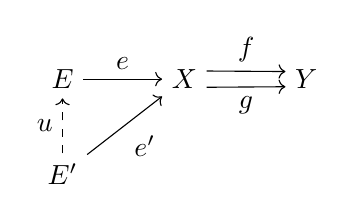
\begin{tikzpicture}
      \node (X) {$X$};
      \node [right=1.0cm of X] (Y) {$Y$};
      \node [left =1.0cm of X] (E) {$E$};
      \node [below=0.7cm of E] (E') {$E'$};
      \draw [->] (X.20) to node [above] {$f$} (Y.160);
      \draw [->] (X.340) to node [below] {$g$} (Y.200);
      \draw [->] (E) to node [above] {$e$} (X);
      \draw [->, dashed] (E') to node [left] {$u$} (E);
      \draw [->] (E') to node [below right] {$e'$} (X);
    \end{tikzpicture}
  \end{center}
\end{definition}

\begin{definition}[余等化子]
  圏 $\cat{J}=\{\cdot\rightrightarrows\cdot\}$ について,
  函手 $F:\cat{J}\to\cat{C}$ の余極限を余等化子 (coequalizer) という.
  \begin{center}
    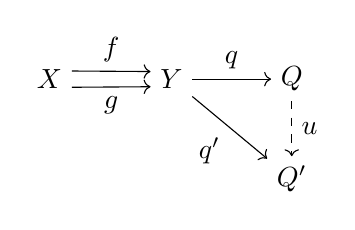
\begin{tikzpicture}
      \node (X) {$X$};
      \node [right=1.0cm of X] (Y) {$Y$};
      \node [right=1.0cm of Y] (Q) {$Q$};
      \node [below=0.7cm of Q] (Q') {$Q'$};
      \draw [->] (X.20) to node [above] {$f$} (Y.160);
      \draw [->] (X.340) to node [below] {$g$} (Y.200);
      \draw [->] (Y) to node [above] {$q$} (Q);
      \draw [->, dashed] (Q) to node [right] {$u$} (Q');
      \draw [->] (Y) to node [below left] {$q'$} (Q');
    \end{tikzpicture}
  \end{center}
\end{definition}

\section{完備}

\begin{definition}[有限完備]
  圏 $\cat{C}$ について任意の有限圏 $\cat{J}$ および函手 $F:\cat{J}\to\cat{C}$
  が極限をもつとき,$\cat{C}$ は有限完備であるという.
\end{definition}

\begin{definition}[完備]
  圏 $\cat{C}$ について任意の小圏 $\cat{J}$ および函手 $F:\cat{J}\to\cat{C}$
  が極限をもつとき,$\cat{C}$ は完備であるという.
\end{definition}

\section{冪}

\begin{definition}[冪]
  \def\C{\cat{C}}%
  \def\a{X}%
  \def\b{Y}%
  \def\c{Z}%
  \def\e{\operatorname{eval}}%
  有限積をもつ圏 $\C$ の対象 $\a,\b,\c\in\objs{\C}$ について,
  対象 $\c^\b\in\objs{\C}$ と射 $\e:\c^\b\times\b\to\c$ の組 $(\c^\b,\e)$ で,
  任意の $f:\a\times\b\to\c$ に対して
  以下の図式を可換にするような射 $\tilde{f}:\a\to\c^\b$ がただ一つ存在するものを
  冪 (exponential) という.
  \begin{center}
    \begin{tikzpicture}
      \node (XY) {$\a\times\b$};
      \node [below=1.0cm of XY] (ZYY) {$\c^{\b}\times\b$};
      \node [right=1.2cm of ZYY] (Z) {$\c$};
      \draw [->] (XY) to node [above right] {$f$} (Z);
      \draw [->, dashed] (XY) to node [left] {$\bar{f}\times\id{\b}$} (ZYY);
      \draw [->] (ZYY) to node [below] {\small$\operatorname{eval}$} (Z);
    \end{tikzpicture}
  \end{center}
\end{definition}

\section{極限の保存}

\begin{definition}[極限の保存]
  \def\C{\cat{C}}%
  \def\D{\cat{D}}%
  \def\f{F}%
  \def\J{\cat{J}}%
  \def\diagram{D}%
  函手 $\mrp{\f}{\C}{\D}$ が
  \begin{equation}
    \forall\J\in\objs{\Cat}\ \forall\diagram\in\Fun{\J}{\C};
    \ \f(\lim(\diagram))\simeq\lim(\f\circ\diagram)
  \end{equation}
  を満たすとき,$\f$ は極限を保存する (preserves limits) という.
\end{definition}

{

\def\C{\cat{C}}%
\def\D{\cat{D}}%
\def\E{\cat{E}}%
\def\c{\obj{c}}%
\def\d{\obj{d}}%
\def\F{F}%
\def\G{G}%
\def\eval{\operatorname{ev}}%

\section{コンマ圏}

\begin{definition}[コンマ圏\cite{nlab:comma_category}]\label{def:comma-category}
  圏 $\C,\D,\E$ と
  区間圏 (\cref{def:interval-category}) $\interval=\{0\to1\}$ および
  函手 $\mrp{\F}{\C}{\E},\mrp{\G}{\D}{\E}$ について,
  $\mrp{\F\times\G}{\C\times\D}{\E\times\E}$ と
  $\eval_0\times\eval_1:\Fun{\interval}{\E}\to\E$ の
  $\Cat$ における引き戻し対象をコンマ圏 (comma category) といい,
  $\Comma{\F}{\G}$ と表記する.
  \begin{center}
    \begin{tikzcd}
      \Comma{\F}{\G}\arrow{r}{}\arrow{d}{}
      & \Fun{\interval}{\E}\arrow{d}{\eval_0\times\eval_1} \\
      \C\times\D\arrow{r}[swap]{\F\times\G}
      & \E\times\E
    \end{tikzcd}
    \begin{tikzcd}
      (\c,\d,\alpha)\arrow[mapsto]{r}\arrow[mapsto]{d}
      & \alpha\arrow[mapsto]{d}{\eval_0\times\eval_1} \\
      (\c,\d)\arrow[mapsto]{r}[swap]{\F\times\G}
      & (\F(\c),\G(\d))
    \end{tikzcd}
  \end{center}
  \begin{center}
    \begin{tikzcd}[column sep=10pt]
      \C\arrow{rrr}{\F}
      &&& \E
      &&& \D\arrow{lll}[swap]{\G} \\
      \c\arrow{d}[swap]{f}
      && \F(\c)\arrow{rr}{\alpha}\arrow{d}[swap]{\F(f)}
      && \G(\d)\arrow{d}{\G(g)}
      && \d\arrow{d}{g} \\
      \c'
      && \F(\c')\arrow{rr}[swap]{\alpha'}
      && \G(\d')
      && \d'
    \end{tikzcd}
  \end{center}
\end{definition}

}

\chapter{表現可能函手}

\section{表現可能函手}

\subsection{hom 函手}

はじめに hom 函手の概念を導入する.
hom 函手は,あるひとつの対象に着目して
そこから見た「主観的な」圏を与える函手である.
共変 hom 函手は他の対象を「そこへの」射の集合と同一視し,
反変 hom 函手は他の対象を「そこからの」射の集合と同一視する.
\begin{definition}[hom 双函手]
  \def\C{\cat{C}}%
  局所小圏 $\C$ について,
  双函手 $\mrp{\C(-,-)}{\op{\C}\times\C}{\set}$
  を hom 双函手 (hom-bifunctor) という.
  ただし $\mrps{\C}{-}{-}$ は
  \begin{itemize}
    \item $a,b\in\C$ を集合 $\mrps{\C}{a}{b}\in\set$ に写し,
    \item $\psi\in\mrps{\C}{a}{a'},\phi\in\mrps{\C}{b}{b'}$
          を以下の写像に写す.
          \begin{equation}
            \mrps{\C}{a'}{b}\in f\mapsto\phi\circ f\circ\psi\in\mrps{\C}{a}{b'}
          \end{equation}
  \end{itemize}
\end{definition}
\begin{definition}[共変 hom 函手]\label{def:covariant-hom-functor}
  \def\C{\cat{C}}%
  \def\c{\obj{c}}%
  局所小圏 $\C$ と対象 $\c\in\objs{\C}$ について,
  hom 双函手の部分適用 $\mrp{\mrps{\C}{\c}{-}}{\C}{\set}$ を
  $\c$ に関する共変 hom 函手 (covariant hom-functor) という.
\end{definition}
\begin{definition}[反変 hom 函手]
  \def\C{\cat{C}}%
  \def\c{\obj{c}}%
  局所小圏 $\C$ と対象 $\c\in\objs{\C}$ について,
  hom 双函手の部分適用 $\mrp{\mrps{\C}{-}{\c}}{\op{\C}}{\set}$ を
  $\c$ に関する反変 hom 函手 (contravariant hom-functor) という.
\end{definition}

\subsection{表現可能函手}

\begin{definition}[前層]
  \def\C{\cat{C}}%
  小圏 $\C$ 上の反変函手 $\op{\C}\to\set$ を
  $\C$ の前層 (presheaf) という.
\end{definition}

表現可能函手とは,
hom 函手に同型な前層のことである.

\begin{definition}[表現可能函手]
  \def\C{\cat{C}}%
  \def\c{\obj{c}}%
  \def\F{F}%
  \def\iso{\phi}%
  小圏 $\C$ の前層 $\F$ と対象 $\c\in\objs{\C}$
  に関する反変 hom 函手 $\mrps{\C}{-}{\c}$ について自然同型
  \begin{equation}
    \iso:\F\cong\mrps{\C}{-}{\c}
  \end{equation}
  が存在するとき,
  $\F$ は表現可能 (representable) であるという.
  このとき $\iso$ を $\F$ の表現 (representation) といい,
  $\c$ を $\F$ の表現対象 (representing object) という.
\end{definition}

\begin{theorem}[hom 函手は極限を保存する]\label{thm:hom-functor-preserves-limits}
  任意の共変 hom 函手 (\cref{def:covariant-hom-functor}) は極限を保存する.
\end{theorem}
\begin{proof}
  \def\C{\cat{C}}%
  \def\c{\obj{c}}%
  \def\f{F}%
  \def\J{\cat{J}}%
  \def\diagram{D}%
  任意の対象 $\c\in\objs{\C}$ および函手 $\mrp{\diagram}{\J}{\C}$ について,
  極限 $\lim(\diagram)$ が存在するならば
  \begin{align}
    \mrps{\C}{\c}{\lim(\diagram)}
     & \simeq\operatorname{Cones}(\c,\diagram) \\
     & \simeq\lim(\mrps{\C}{\c}{\diagram(-)}).
  \end{align}
  ただし $\operatorname{Cones}(\c,\diagram)$ は
  $\c$ から $\diagram$ への錐の全体を表す.
\end{proof}

\section{米田の補題}

\subsection{米田埋め込み}

\begin{definition}[米田埋め込み]
  \def\C{\cat{C}}%
  局所小圏 $\C$ について,
  hom 双函手 $\mrp{\C(-,-)}{\op{\C}\times\C}{\set}$ の左カリー化
  $\mrp{\yoneda}{\C}{\set^{\op{\C}}}$ を米田埋め込み (Yoneda embedding) という.
  \begin{center}
    \begin{tikzpicture}
      % Set
      \node (s) {$\set$};
      \node [below right=0.1cm and -1.5cm of s] (scom) {
        \begin{tikzcd}[row sep=1.0cm, column sep=1.5cm]
          \mrps{\cat{C}}{x}{a}\arrow{d}{\psi\circ-}[swap]{\mrps{\cat{C}}{x}{\psi}}
          & \mrps{\cat{C}}{y}{a}\arrow{l}{-\circ\phi}[swap]{\mrps{\cat{C}}{\phi}{a}}
          \arrow{d}{\mrps{\cat{C}}{y}{\psi}}[swap]{\psi\circ-} \\
          \mrps{\cat{C}}{x}{b}
          & \mrps{\cat{C}}{y}{b}\arrow{l}{\mrps{\cat{C}}{\phi}{b}}[swap]{-\circ\phi}
        \end{tikzcd}
      };
      \node [above left = 0.1cm and  0.5cm of s]    (srec1) {};
      \node [below right=-0.1cm and -0.2cm of scom] (srec2) {};
      \draw [draw=blue!70,rounded corners=10] (srec1) rectangle (srec2);

      % source category
      \node [left=4.0cm of s]     (opc) {$\op{\C}$};
      \node [above=1.2cm of opc]  (c)   {$\C$};
      \node [above=0.5cm of c]    (y)   {$y$};
      \node [left =0.4cm of y]    (x)   {$x$};
      \node [below=0.1cm of x]    (a)   {$a$};
      \node [below=0.3cm of a]    (b)   {$b$};
      \draw [->] (a) to node [right] {\scriptsize$\psi$} (b);
      \draw [->] (x) to node [above] {\scriptsize$\phi$} (y);
      \node [above left =0.2cm and 0.1cm of x] (crec1) {};
      \node [below right=0.2cm and 0.1cm of c] (crec2) {};
      \draw [draw=gray,rounded corners=10] (crec1) rectangle (crec2);

      % functor category
      \node [right=1.7cm of c] (f) {${\set}^{\op{\C}}$};
      \draw [->, bend left =20] (opc) to node (ya) [above] {$\mrps{\C}{-}{a}$} (s);
      \draw [->, bend right=20] (opc) to node (yb) [below] {$\mrps{\C}{-}{b}$} (s);
      \draw [->, double] (ya) to node [right] {\scriptsize$\mrps{\C}{-}{\psi}$} (yb);
      \draw [->] (c) to node [right] {$\mathrm{id}^\mathrm{op}_\C$} (opc);
      \draw [->] (c) to node [above left=0cm and -0.1cm] {$\textbf{よ}$} (f);
      \node [above left =0.0cm and 0.5cm of f] (frec1) {};
      \node [below right=0.0cm and 0.4cm of yb] (frec2) {};
      \draw [draw=red!60,rounded corners=10] (frec1) rectangle (frec2);
    \end{tikzpicture}
  \end{center}
\end{definition}
\begin{definition}[余米田埋め込み]
  \def\C{\cat{C}}%
  局所小圏 $\C$ について,
  hom 双函手 $\mrp{\C(-,-)}{\op{\C}\times\C}{\set}$ の右カリー化
  $\mrp{\yoneda'}{\op{\C}}{\set^{\C}}$ を余米田埋め込み (coYoneda embedding) という.
  \begin{center}
    \begin{tikzpicture}
      % Set
      \node (s) {$\set$};
      \node [below right=0.1cm and -1.5cm of s] (scom) {
        \begin{tikzcd}[row sep=1.0cm, column sep=1.5cm]
          \mrps{\cat{C}}{a}{x}\arrow{r}{\mrps{\cat{C}}{a}{\psi}}[swap]{-\circ\phi}
          & \mrps{\cat{C}}{a}{y} \\
          \mrps{\cat{C}}{b}{x}\arrow{r}{\phi\circ-}[swap]{\mrps{\cat{C}}{b}{\phi}}\arrow{u}{\mrps{\cat{C}}{\psi}{x}}[swap]{\psi\circ-}
          & \mrps{\cat{C}}{b}{y}\arrow{u}{-\circ\psi}[swap]{\mrps{\cat{C}}{\psi}{y}}
        \end{tikzcd}
      };
      \node [above left = 0.1cm and  0.5cm of s]    (srec1) {};
      \node [below right=-0.1cm and -0.2cm of scom] (srec2) {};
      \draw [draw=blue!70,rounded corners=10] (srec1) rectangle (srec2);

      % source category
      \node [left =4.0cm of s] (c)   {$\C$};
      \node [above=1.2cm of c] (opc) {$\op{\C}$};
      \node [below=0.7cm of c] (y)   {$y$};
      \node [left =0.4cm of y] (x)   {$x$};
      \node [above=0.1cm of x] (b)   {$b$};
      \node [above=0.3cm of b] (a)   {$a$};
      \draw [->] (a) to node [right] {\scriptsize$\psi$} (b);
      \draw [->] (x) to node [above] {\scriptsize$\phi$} (y);
      \node [above left =0.0cm and 0.1cm of a] (crec1) {};
      \node [below right=0.0cm and 0.1cm of y] (crec2) {};
      \draw [draw=gray,rounded corners=10] (crec1) rectangle (crec2);

      % functor category
      \node [right=1.5cm of opc] (f) {$\set^\C$};
      \draw [->, bend left =20] (c) to node (ya) [above] {$\mrps{\C}{a}{-}$} (s);
      \draw [->, bend right=20] (c) to node (yb) [below] {$\mrps{\C}{b}{-}$} (s);
      \draw [->, double] (ya) to node [right] {\scriptsize$\mrps{\C}{\psi}{-}$} (yb);
      \draw [->] (c) to node [right] {$\mathrm{id}^\mathrm{op}_\C$} (opc);
      \draw [->] (opc) to node [above left=0cm and -0.1cm] {$\textbf{よ}'$} (f);
      \node [above left =0.0cm and 0.5cm of f] (frec1) {};
      \node [below right=0.0cm and 0.4cm of yb] (frec2) {};
      \draw [draw=red!60,rounded corners=10] (frec1) rectangle (frec2);
    \end{tikzpicture}
  \end{center}
\end{definition}

{

\def\C{\cat{C}}%
\def\diagram{D}%
\def\c{\obj{c}}%
\def\eval{\operatorname{ev}}%

\begin{theorem}\label{thm:yepl-lemma}%
  \def\J{\cat{J}}%
  \def\D{\cat{D}}%
  任意の小圏 $\C,\J$ ,局所小圏 $\D$ および函手
  $\mrp{\diagram}{\J}{\Fun{\C}{\D}}$ を考える.
  各 $\c\in\objs{\C}$ における評価函手 $\eval_{\c}:\Fun{\C}{\D}\to\D$
  について極限 $\lim(\eval_{\c}\circ\diagram)$ が存在するならば,
  極限 $\lim(\diagram)$ が存在し,
  \begin{equation}
    \forall\c\in\objs{\C};
    \ (\lim\diagram)(c)\simeq\lim(\eval_{\c}\circ\diagram).
  \end{equation}
\end{theorem}

\begin{theorem}[米田埋め込みは極限を保存する]
  任意の局所小圏 $\C$ について,
  米田埋め込み $\mrp{\yoneda}{\C}{\set^{\op{\C}}}$ は極限を保存する.
\end{theorem}

\begin{proof}
  \begin{align}
    \yoneda(\lim\diagram)(\c)
     & \simeq\mrps{\C}{\c}{\lim\diagram}                             \\
     & \simeq\lim(\yoneda'(c)\circ\diagram)\label{yepl-2}            \\
     & \simeq\lim(\eval_{\c}\circ\yoneda\circ\diagram)\label{yepl-3} \\
     & \simeq\lim(\yoneda\circ\diagram)(\c)\label{yepl-4}.
  \end{align}
  ただし \cref{yepl-2} の同型は \cref{thm:hom-functor-preserves-limits} による.
  また \cref{yepl-3} の同型は
  $\yoneda'(\c)=\mrps{\C}{\c}{-}=\eval_{\c}\circ\yoneda$
  によって得られ,
  \cref{yepl-4} の同型は \cref{thm:yepl-lemma} による.
\end{proof}
}

{

\subsection{米田の補題}

\def\C{\cat{C}}%
\def\opC{\op{\C}}%
\def\c{\obj{c}}%
\def\d{\obj{c}'}%
\def\K{K}%

所与の前層 $\mrp{\K}{\C}{\set}$ に対して
表現可能函手 $\yoneda(\c)$ からの自然変換 $\alpha$ を与えることは,
コンポーネント ${\alpha}_{\c}$ が恒等射 $\id{\c}$
をどこに写すかを決めることと等価である.
以下で紹介する米田の補題 (Yoneda lemma) はその事実を主張しており,
${\alpha}_{\c}(\id{\c})$ の値ひとつから自然変換 $\alpha$ を構成する方法を提供する.

\begin{theorem}[米田の補題]
  $\C$ を局所小圏とする.
  任意の前層 $\mrp{\K}{\opC}{\set}$ と $\c\in\objs{\C}$ について
  \begin{equation}
    y:\set^{\opC}(\yoneda(\c),\K)\ni\alpha\mapsto\alpha_{\c}(\id{\c})\in\K(\c)
  \end{equation}
  は全単射である.
\end{theorem}
\begin{proof}
  \def\a{\obj{a}}%
  $\mrp{x}{K(\c)}{\set^\C(\mrps{\C}{\c}{-},K)}$ を考え,
  $x$ が $\set$ における $y$ の逆射であることを示す.
  ただし $x$ は任意の $\a\in K(\c)$ を以下のコンポーネントで構成される自然変換
  $x(\a)$ に写す:
  \begin{equation}
    {x(\a)}_{\d}:f\mapsto K(f)(\a).
  \end{equation}
  $y\circ x=\id{K(\c)}$ を示す.任意の $\a\in K(\c)$ について
  \begin{align*}
    y(x(\a)) & ={x(\a)}_{\c}(\id{\c}) \\
             & =K(\id{\c})(\a)        \\
             & =\id{K(\c)}(\a)        \\
             & =\a.
  \end{align*}
  $x\circ y=\id{\set^\C(\mrps{\cat{D}}{\c}{-},K)}$ を示す.
  任意の $\alpha:\mrps{\C}{\c}{\d}\to K$,$\d\in\objs{\C}$,
  $\mrp{f}{\c}{\d}$ について
  \begin{align*}
    {x(y(\alpha))}_{\d}(f) & =K(f)(y(\alpha))                        \\
                           & =K(f)(\alpha_{\c}(\id{\c}))             \\
                           & =\alpha_{\d}(\mrps{\C}{\c}{f}(\id{\c})) \\
                           & =\alpha_{\d}(f).
  \end{align*}
  ここで 3 行目の変換には,以下の図式が可換である事実を用いた.
  \begin{center}
    \begin{tikzcd}
      \mrps{\C}{\c}{\c}\arrow{r}{\mrps{\C}{\c}{f}}\arrow{d}[swap]{\alpha_{\c}}
      & \mrps{\C}{\c}{\d}
      \arrow{d}{\alpha_{\d}} \\
      \K(\c)\arrow{r}[swap]{\K(f)} & \K(\d)
    \end{tikzcd}
  \end{center}
  よって $y$ は全単射であることが示された.
\end{proof}

\subsection{米田の補題の系}

\begin{theorem}[米田埋め込みは充満忠実]
  任意の局所小圏 $\C$ において
  米田埋め込み $\mrp{\yoneda}{\C}{\set^{\op{\C}}}$ は充満忠実
  (\cref{def:full-faithful}) である.
\end{theorem}
\begin{proof}
  \def\x{\obj{x}}%
  \def\y{\obj{y}}%
  米田の補題より,任意の $\x,\y\in\objs{\C}$ について
  \begin{equation}
    \set^{\op{\C}}(\yoneda(\x),\yoneda(\y))
    \simeq\yoneda(\y)(\x)
    \simeq\mrps{\C}{\x}{\y}.
  \end{equation}
\end{proof}

\begin{theorem}[表現対象の一意性]\label{thm:unique-representable-object}
  任意の小圏 $\C$ について
  \begin{equation}
    \forall\c,\d\in\objs{\C};\ \c\simeq\d\iff\yoneda(\c)\simeq\yoneda(\d).
  \end{equation}
\end{theorem}

\begin{theorem}[Cayley の定理]
  任意の群 $G$ は,対称群 $\operatorname{Sym}(G)$ の部分群と同型である.
\end{theorem}

\subsection{任意の前層は表現可能函手の余極限として書ける}

\def\psh{P}%

\begin{definition}[要素の圏]
  前層 $\mrp{\psh}{\op{\C}}{\set}$ および
  $\C$ の終対象 $\mrp{1}{\mathbf{1}}{\set}$ について,
  コンマ圏 (\cref{def:comma-category}) $\op{\Comma{1}{\psh}}$ を
  $\psh$ の要素の圏 (category of elements) といい,
  $\Elem{\C}{\psh}$ と表記する.
  \begin{center}
    \begin{tikzcd}[column sep=8pt]
      &
      \set
      &
      &
      & \Elem{\C}{\psh} \\
      1\arrow[equal]{d}\arrow{rr}{x}
      &
      & \psh(c)
      &
      & \langle c,x\rangle\arrow{d}{f} \\
      1\arrow{rr}[swap]{x'}
      &
      & \psh(c')\arrow{u}[swap]{\psh(f)}
      &
      & \langle c',x'\rangle
    \end{tikzcd}
  \end{center}
\end{definition}

\begin{theorem}[任意の前層は表現可能函手の余極限として書ける]
  任意の前層 $\mrp{\psh}{\op{\C}}{\set}$ について,
  表現可能函手 $\mrp{F}{\Elem{\C}{\psh}}{\set}$ が存在して
  \begin{equation}
    \psh\simeq\colim(F).
  \end{equation}
\end{theorem}

\begin{proof}
  米田の補題より,
  任意の $\langle c,x\rangle\in\objs{\Elem{\C}{\psh}}$ について,
  $x\in\psh(c)$ に対応する自然変換 $\phi_{\langle c,x\rangle}$ が存在する.

  (i) 各 $\langle c,x\rangle\in\objs{\Elem{\C}{\psh}}$ について
  $\phi_{\langle c,x\rangle}$ をコンポーネントとする $\phi$ が
  自然変換であることを示す.
  すなわち,
  任意の $\mrp{f}{\langle c,x\rangle}{\langle c',x'\rangle}$ および
  $d\in\objs{\C}$ について以下の図式が可換であることを示す:
  \begin{center}
    \begin{tikzcd}
      \psh(d)\arrow[equal]{r}
      & \psh(d) \\
      \mrps{\C}{d}{c}
      \arrow{u}{\left(\phi_{\langle c,x\rangle}\right)_{d}}\arrow{r}{\yoneda(f)}
      & \mrps{\C}{d}{c'}\arrow{u}[swap]{\left(\phi_{\langle c',x'\rangle}\right)_{d}}.
    \end{tikzcd}
  \end{center}
  任意の $\mrp{g}{d}{c}$ について
  \begin{align*}
    {\left(\phi_{\langle c',x'\rangle}\right)}_{d}(\yoneda(f)(g))
     & ={\left(\phi_{\langle c',x'\rangle}\right)}_{d}(f\circ g) \\
     & =\psh(f\circ g)(x')                                       \\
     & =\psh(g)(\psh(f)(x'))                                     \\
     & =\psh(g)(x)                                               \\
     & ={\left(\phi_{\langle c,x\rangle}\right)}_{d}(g).
  \end{align*}
  よって自然変換 $\mrp{\phi}{F}{\Delta(\psh)}$ が得られ,
  $(\Delta(\psh),\phi)$ は $F$ からの余錐であることが示された.

  (ii) $(\Delta(\psh),\phi)$ が $F$ の余極限であることを示す.
  まず,$F$ からの任意の余錐 $(\Delta(Q),\psi)$ に対して,
  以下に定められる写像の族
  ${\{\mu_{c}\}}_{c\in\objs{\C}}$
  が自然変換であることを示す:
  \begin{equation}
    \mu_{c}:\psh(c)\ni x\mapsto
    {\left(\psi_{\langle c,x\rangle}\right)}_{c}(\id{c})\in Q(c).
  \end{equation}
  任意の $\mrp{f}{\langle c,x\rangle}{\langle c',x'\rangle}$ について
  \begin{align*}
    \mu_{c}(\psh(f)(x'))
     & =\mu_{c}(x)                                                                \\
     & ={\left(\psi_{\langle c,x\rangle}\right)}_{c}(\id{c})                      \\
     & ={\left(\psi_{\langle c',x'\rangle}\right)}_c(f)                           \\
     & =Q(f)\left({\left(\psi_{\langle c',x'\rangle}\right)}_{c'}(\id{c'})\right) \\
     & =Q(f)(\mu_{c'}(x')).
  \end{align*}
  次に,$\psi=\mu\circ\phi$ であることを示せばよい.
  任意の
  $\langle c,x\rangle\in\objs{\Elem{\C}{\psh}},d\in\objs{\C},\mrp{g}{d}{c}$
  について
  \begin{align*}
    \mu_{d}\circ{\left(\phi_{\langle c,x\rangle}\right)}_{d}(g)
     & =\mu_{d}(\psh(g)(x))                                                   \\
     & =Q(g)(\mu_{c}(x))                                                      \\
     & =Q(g)\left({\left(\psi_{\langle c,x\rangle}\right)}_{c}(\id{c})\right) \\
     & ={\left(\psi_{\langle c,x\rangle}\right)}_{d}(g).
  \end{align*}
\end{proof}

}

\chapter{随伴}

\section{随伴}

\begin{definition}[随伴]
  \def\C{\cat{C}}%
  \def\D{\cat{D}}%
  \def\L{L}%
  \def\R{R}%
  函手 $\mrp{\L}{\C}{\D},\mrp{\R}{\D}{\C}$ について自然同型
  \begin{equation}
    \mrps{\D}{\L(-)}{-}\simeq\mrps{\C}{-}{\R(-)}
  \end{equation}
  が存在するとき $\L$ と $\R$ は随伴 (adjoint) であるといい,
  $\L\dashv\R$ と表記する.
  またこのとき $\L$ を $\R$ の左随伴 (left adjoint) といい,
  $\R$ を $\L$ の右随伴 (right adjoint) という.
\end{definition}

\begin{theorem}[随伴函手の並列定義]\label{thm:adjoint-functor-definitions}
  函手 $F:\cat{C}\rightleftarrows\cat{D}:G$ について以下の命題は全て同値である:
  \begin{enumerate}
    \item $F\dashv G$.
    \item 自然変換 $\eta:\id{\cat{C}}\to GF$ が存在し,
          各 $\eta_c:c\to GF(c)$ が $c$ から $G$ への普遍射である.
    \item 自然変換 $\epsilon:FG\to\id{\cat{D}}$ が存在し,
          各 $\epsilon_d:FG(d)\to d$ が $F$ から $d$ への普遍射である.
  \end{enumerate}
\end{theorem}

\subsection{随伴函手の例}

{
  \def\C{\cat{C}}%
  \begin{theorem}[終対象]
    任意の圏 $\C$ において以下は同値である:
    \begin{enumerate}[label=(\roman*)] % chktex 36
      \item $\C$ が終対象をもつ,
      \item 一意な函手 $*:\C\to\mathbf{1}$ が右随伴をもつ.
    \end{enumerate}
  \end{theorem}
  \begin{proof}
    \def\c{\obj{c}}%
    自明な函手 $\mrp{\phi}{\mathbf{0}}{\C}$ および
    任意の函手 $t:\mathbf{1}\to\C$ について
    \begin{align} % chktex 36
      t(*)\simeq\lim(\phi)
       & \iff\forall\c\in\objs{\C};
      \ |\mrps{\C}{c}{t(*)}|=1                                   \\
       & \iff\mrps{\C}{-}{t(-)}\simeq\mrps{\mathbf{1}}{*(-)}{-}.
    \end{align}
    よって (i) $\Leftrightarrow$ (ii) が示された.
  \end{proof}
}

\begin{theorem}[積函手と冪函手]
  \begin{equation}
    -\times A\dashv{(-)}^A.
  \end{equation}
\end{theorem}

\begin{proof}
  \cref{thm:adjoint-functor-definitions} の (i) $\Leftrightarrow$ (iii) を用いる.
  評価射 $\epsilon_c:{C}^A\to C$ が
  (i) 対象 $C$ について自然であり,
  (ii) $-\times A$ から $C$ への普遍射であることを示す.

  \begin{enumerate}[label=(\roman*)] % chktex 36
    \item 自然性を示す.
          冪函手の定義より,任意の $C,D\in\objs{\cat{C}}$ と射 $f:C\to D$ について
          \begin{align*}
            f\circ\epsilon_C
             & =\epsilon_D\circ(\widetilde{(f\circ\epsilon_C)}\times\id{A}) \\
             & =\epsilon_D\circ(f^A\times\id{A})                            \\
          \end{align*}
          よって自然性は示された.
    \item 普遍性を示す.
          冪函手の定義より,任意の $X\in\objs{\cat{C}}$ と $g:X\times A\to C$
          について以下を満たす$\tilde{g}:X\to C^A$ がただ一つ存在する:
          \begin{equation*}
            \epsilon_C\circ(\tilde{g}\times\id{A})=g.
          \end{equation*}
          よって普遍性は示された.
  \end{enumerate}
\end{proof}

\subsection{随伴は極限を保存する}

{
  \def\C{\cat{C}}%
  \def\D{\cat{D}}%
  \def\E{\cat{E}}%
  \def\L{L}%
  \def\R{R}%
  \def\F{F}%
  \def\d{d}%
  \begin{theorem}[右随伴は極限を保存する]
    $\L\dashv\R$ のとき,任意の圏 $\C,\D,\E$ について
    \begin{equation}
      \forall\L\in\objs{\Fun{\C}{\D}}\ \forall\R\in\objs{\Fun{\D}{\C}};
      \ \L\dashv\R\rightarrow\left(
      \forall\F\in\objs{\Fun{\C}{\E}};\ \R(\lim{\F})\simeq\lim(\R\F)
      \right).
    \end{equation}
  \end{theorem}
  \begin{proof}
    任意の $\d\in\objs{\D}$ について
    \begin{align}
      \mrps{\D}{\d}{\R(\lim(F))}
       & \simeq\mrps{\C}{\L(\d)}{\lim(F)}                   \\
       & \simeq\lim\mrps{\C}{\L(\d)}{F(-)}\label{eq:rapl-2} \\
       & \simeq\lim\mrps{\D}{\d}{RF(-)}                     \\
       & \simeq\mrps{\D}{\d}{\lim(RF)}
    \end{align}
    ただし \cref{eq:rapl-2} では \cref{thm:hom-functor-preserves-limits}
    を用いた.
    よって \cref{thm:unique-representable-object} より $\R(\lim(F))\simeq\lim(RF)$.
  \end{proof}
}

{

  \def\C{\cat{C}}%
  \def\D{\cat{D}}%
  \def\E{\cat{E}}%
  \def\i{1}%
  \def\F{F}%
  \def\G{G}%
  \def\w{\obj{w}}%
  \def\x{\obj{x}}%
  \def\y{\obj{y}}%
  \def\z{\obj{z}}%
  \def\monad{M}%

  \chapter{モナドと代数}

  \section{モナド}

  \begin{definition}[モノイド圏]\label{def:monoidal-category}
    圏 $\C$ ,双函手 $\mrp{\otimes}{\C\times\C}{\C}$ ,対象 $\i\in\objs{\C}$
    および以下の 3 つの自然同型
    \begin{align}
      \alpha  & :(-\otimes-)\otimes-\simeq-\otimes(-\otimes-), \\
      \lambda & :\i\otimes-\simeq\id{\C},                      \\
      \rho    & :-\otimes\i\simeq\id{\C}
    \end{align}
    が任意の $\w,\x,\y,\z\in\objs{\C}$ について
    以下の 2 つの図式を可換にするとき,
    $(\C,\otimes,\i,\alpha,\lambda,\rho)$
    をモノイド圏 (monoidal category) という.
    \begin{center}
      \begin{tikzcd}
        (\x\otimes\i)\otimes\y
        \arrow{rr}{\alpha_{\x,\i,\y}}
        \arrow{rd}[swap]{\rho_x\times\id{\y}}
        &
        & \x\otimes(\i\times\y)
        \arrow{ld}{\id{\x}\otimes\lambda_y} \\
        & \x\otimes\y
      \end{tikzcd}
    \end{center}
    \begin{center}
      \begin{tikzcd}
        & (\w\otimes\x)\otimes(\y\otimes\z)
        \arrow{rd}{\alpha_{\w,\x,\y\otimes\z}} \\
        ((\w\otimes\x)\otimes\y)\otimes\z
        \arrow{ru}{\alpha_{\w\otimes\x,\y,\z}}
        \arrow{d}{\alpha_{\w,\x,\y}\otimes\id{\z}}
        &
        & \w\otimes(\x\otimes(\y\otimes\z)) \\
        (\w\otimes(\x\otimes\y))\otimes\z
        \arrow{rr}{\alpha_{\w,\x\otimes\y,\z}}
        &
        & \w\otimes((\x\otimes\y)\otimes\z)
        \arrow{u}{\id{\w}\otimes\alpha_{\x,\y,\z}}
      \end{tikzcd}
    \end{center}
  \end{definition}

  \begin{definition}[モノイド]
    モノイド圏 $(\C\otimes,\i,\alpha,\lambda,\rho)$ ,
    対象 $\monad\in\objs{\C}$ および
    射 $\mrp{\mu}{\monad\times\monad}{\monad},\mrp{\eta}{\i}{\monad}$
    が以下の 2 つの図式を可換にするとき,
    $(\monad,\mu,\eta)$ を $\C$ におけるモノイド (monoid) または
    モノイド対象という.
    \begin{center}
      \begin{tikzcd}[column sep=10pt]
        & (\monad\otimes\monad)\otimes\monad%
        \arrow{rr}{\alpha}\arrow{ld}[swap]{\mu\otimes\i}
        && \monad\otimes(\monad\otimes\monad)
        \arrow{rd}{\i\otimes\mu} \\
        \monad\otimes\monad%
        \arrow{rr}[swap]{\mu}
        && \monad%
        && \monad\otimes\monad%
        \arrow{ll}{\mu} \\
      \end{tikzcd}
    \end{center}
    \begin{center}
      \begin{tikzcd}[column sep=40pt]
        \i\otimes\monad%
        \arrow{r}{\eta\otimes\id{\monad}}\arrow{rd}[swap]{\lambda_{\monad}}
        & \monad\otimes\monad%
        & \monad\otimes\i
        \arrow{l}[swap]{\id{\monad}\otimes\eta}
        \arrow{ld}{\rho_{\monad}} \\
        & \monad%
      \end{tikzcd}
    \end{center}
  \end{definition}

  \begin{definition}[モナド]
    圏 $\C$ について,
    モノイド圏としての $\C$ の自己函手圏
    $(\Fun{\C}{\C},\circ,\id{\C})$
    におけるモノイド $(\monad,\eta,\mu)$ を
    $\C$ におけるモナド (monad) という.
  \end{definition}

  \subsection{随伴とモナド}

  \begin{theorem}[随伴はモナドを構成する]
    任意の随伴 $(\mrp{F}{\C}{\D},\mrp{\G}{\D}{\C},\eta,\epsilon)$ について,
    $(\G\circ\F,\eta,\G\circ\epsilon\circ\F)$ は $\C$ 上のモナドである.
  \end{theorem}
}

\chapter{カン拡張}

\epigraph{All Concepts are Kan Extensions.}{Saunders Mac Lane}

\section{カン拡張}

カン拡張とは,写像の定義域をより大きな空間へ拡張する操作の一般化である.

\subsection{大域的なカン拡張}

最初に,大域的なカン拡張の定義を与える.

\begin{definition}[函手の誘導]
  \def\C{\cat{C}}%
  \def\A{\cat{C'}}%
  \def\D{\cat{D}}%
  \def\K{K}%
  \def\h{H}%
  函手 $\mrp{\K}{\C}{\A}$ および圏 $\D$ について,
  以下のように定義される函手 $\mrp{\K^*}{\D^\A}{\D^\C}$ を
  $\K$ と $\D$ によって誘導される函手という:
  \begin{align}
    \objs{\D^\A}\ni\h
     & \mapsto\h\circ\K\in\objs{\D^\C},                            \\
    \mrps{\D^\A}{\h}{\h'}\ni\sigma
     & \mapsto\sigma\circ\K\in\mrps{\D^\C}{\h\circ\K}{\h'\circ\K}.
  \end{align}
\end{definition}
\begin{definition}[(大域的な) 左カン拡張]
  \def\C{\cat{C}}%
  \def\A{\cat{C'}}%
  \def\D{\cat{D}}%
  \def\K{K}%
  \def\L{\K_!}%
  函手 $\mrp{\K}{\C}{\A}$ および圏 $\D$ によって誘導される函手
  $\mrp{\K^*}{\D^\A}{\D^\C}$ が左随伴 $\mrp{\L}{\D^\C}{\D^\A}$ をもつとき,
  $\L$ を $\K$ に沿った左カン拡張 (left Kan extension) といい,
  $\L=\lan_{\K}$ と表記する.
\end{definition}
\begin{definition}[(大域的な) 右カン拡張]
  \def\C{\cat{C}}%
  \def\A{\cat{C'}}%
  \def\D{\cat{D}}%
  \def\K{K}%
  \def\R{\K_*}%
  函手 $\mrp{\K}{\C}{\A}$ および圏 $\D$ によって誘導される函手
  $\mrp{\K^*}{\D^\A}{\D^\C}$ が右随伴 $\mrp{\R}{\D^\C}{\D^\A}$ をもつとき,
  $\R$ を $\K$ に沿った右カン拡張 (right Kan extension) といい,
  $\R=\ran_{\K}$ と表記する.
\end{definition}

\subsection{局所的なカン拡張}

\begin{definition}[(局所的な) 左カン拡張]
  \def\C{\cat{C}}%
  \def\A{\cat{C'}}%
  \def\D{\cat{D}}%
  \def\K{K}%
  \def\f{F}%
  函手 $\mrp{\K}{\C}{\A}$ および圏 $\D$ によって誘導される函手
  $\mrp{\K^*}{\D^\A}{\D^\C}$ と函手 $\mrp{\f}{\C}{\D}$ について,
  集合値函手 $\mrp{\mrps{\D^\C}{\f}{\K^*(-)}}{\D^\A}{\set}$ が表現可能であるとき,
  その表現対象 $L\in\objs{\D^\A}$ を $\K$ に沿った $\f$ の左カン拡張といい,
  $L=\lan_{\K}\f$ と表記する.
  \begin{center}
    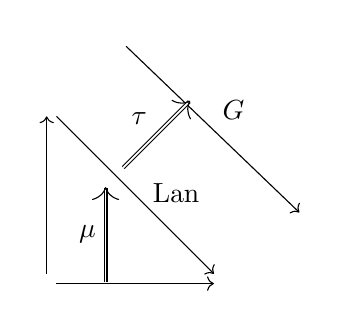
\begin{tikzpicture}
      \def\L{\K_!}%
      \def\g{G}%
      \node (C) {$\A$};
      \node [below=2cm of C] (M) {$\C$};
      \node [right=2cm of M] (A) {$\D$};
      \draw [->] (M) to node [left]         {$\K$}      (C);
      \draw [->] (M) to node [below]        {$\f$}      (A);
      \draw [->] (C) to node [right=0.1cm]  {$\lan_{\K}\f$} (A);
      \node [above right=0.9cm of C] (astart) {};
      \node [below right=2.1cm and 2.2cm of astart] (aend) {};
      \draw [->] (astart) to node [above right] {$\g$} (aend);
      \node [below right=0.65cm and 0.5cm of C] (eend) {};
      \node [below=1.2cm of eend] (estart) {};
      \draw [->,double] (estart) to node [left] {$\mu$} (eend);
      \node [above right=1.1cm and 0.6cm of M] (sstart) {};
      \node [above right=1.2cm of sstart] (send) {};
      \draw [->,double] (sstart) to node [above left] {$\tau$} (send);
    \end{tikzpicture}
  \end{center}
\end{definition}

\begin{definition}[(局所的な) 右カン拡張]
  \def\C{\cat{C}}%
  \def\A{\cat{C'}}%
  \def\D{\cat{D}}%
  \def\K{K}%
  \def\f{F}%
  函手 $\mrp{\K}{\C}{\A}$ および圏 $\D$ によって誘導される函手
  $\mrp{\K^*}{\D^\A}{\D^\C}$ と函手 $\mrp{\f}{\C}{\D}$ について,
  集合値函手 $\mrp{\mrps{\D^\C}{\K^*(-)}{\f}}{\D^\A}{\set}$ が表現可能であるとき,
  その表現対象 $R\in\objs{\D^\A}$ を $\K$ に沿った $\f$ の右カン拡張といい,
  $R=\ran_{\K}\f$ と表記する.
  \begin{center}
    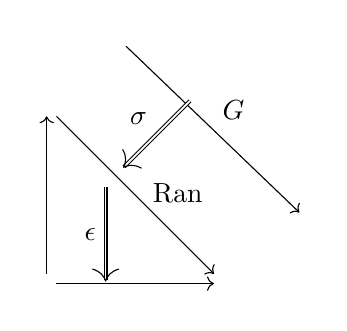
\begin{tikzpicture}
      \def\R{\K_*}%
      \def\g{G}%
      \node (C) {$\A$};
      \node [below=2cm of C] (M) {$\C$};
      \node [right=2cm of M] (A) {$\D$};
      \draw [->] (M) to node [left]         {$\K$}      (C);
      \draw [->] (M) to node [below]        {$\f$}      (A);
      \draw [->] (C) to node [right=0.1cm]  {$\ran_{\K}\f$} (A);
      \node [above right=0.9cm of C] (astart) {};
      \node [below right=2.1cm and 2.2cm of astart] (aend) {};
      \draw [->] (astart) to node [above right] {$\g$} (aend);
      \node [below right=0.65cm and 0.5cm of C] (estart) {};
      \node [below=1.2cm of estart] (eend) {};
      \draw [->,double] (estart) to node [left] {$\epsilon$} (eend);
      \node [above right=1.1cm and 0.6cm of M] (send) {};
      \node [above right=1.2cm of send] (sstart) {};
      \draw [->,double] (sstart) to node [above left] {$\sigma$} (send);
    \end{tikzpicture}
  \end{center}
\end{definition}

\subsection{カン拡張の例}

\begin{theorem}[米田埋め込みのカン拡張]
  \def\C{\cat{C}}%
  \def\A{\C'}%
  \def\K{K}%
  \def\x{\obj{x}}%
  任意の小圏 $\C$ ,圏 $\A$ および函手 $\mrp{\K}{\C}{\A}$ について
  \begin{equation}
    \forall\x\in\objs{\A};\ (\lan_{\K}\yoneda_{\C})(x)\simeq\yoneda_{\A}(\x)\circ\K.
  \end{equation}
\end{theorem}

\subsection{絶対カン拡張}

{
  \def\C{\cat{C}}%
  \def\A{\cat{C'}}%
  \def\D{\cat{D}}%
  \def\E{\cat{E}}%
  \def\K{K}%
  \def\F{F}%
  \def\G{G}%
  \begin{definition}[函手と左カン拡張の交換]
    函手 $\mrp{\K}{\C}{\A}$ に沿った函手 $\mrp{\F}{\C}{\D}$ の左カン拡張
    $\lan_{\K}\F$ および函手 $\mrp{\G}{\D}{\E}$ について
    \begin{equation}
      \lan_{\K}(\G\circ\F)\simeq\G\circ\lan_{\K}\F
    \end{equation}
    が成り立つとき,
    $\G$ は $\lan_{\K}\F$ と交換するという.
  \end{definition}
  \begin{definition}[絶対左カン拡張]
    函手 $\mrp{\K}{\C}{\A}$ に沿った函手 $\mrp{\F}{\C}{\D}$ の左カン拡張
    $\lan_{\K}\F$ について,
    任意の圏 $\E$ および函手 $\mrp{\G}{\D}{\E}$ が
    $\lan_{\K}\F$ と交換するとき,
    $\lan_{\K}\F$ を絶対左カン拡張 (absolute left Kan extension) という.
  \end{definition}
}

\section{すべての概念はカン拡張である}

本節では,極限や随伴がカン拡張として表現されることを確認する.

\begin{theorem}[%
    極限は右カン拡張である\cite{maclane:kan-extensions}%
  ]\label{thm:limit-is-right-kan-extension}
  函手 $T:\cat{M}\to\cat{A}$ について以下の2つは同値である:
  \begin{itemize}
    \item $T$ が極限をもつ,
    \item $T$ が (一意的な) 函手 $K_1:\cat{M}\to\mathbf{1}$
          に沿った右カン拡張をもつ.
  \end{itemize}
  またこれらが成り立つとき $\lim T\simeq\ran_{K_1}T$.
\end{theorem}

\begin{proof}
  函手 $A:\mathbf{1}\to\cat{A}$ は $\cat{A}$ の対象であり,
  $A\circ K_1=\Delta(A)$ である.
  よって自然変換 $\alpha:A\circ K_1\to T$ は $T$ への錐 $(A,\alpha)$ をなす.
  右カン拡張 $(\ran_{K_1}T,\epsilon)$ も同様に $T$ への錐であり,
  その定義より極限錐に同型である.
\end{proof}

\begin{center}
  \begin{minipage}[b]{0.4\linewidth}
    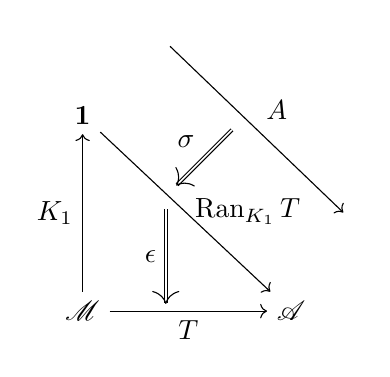
\begin{tikzpicture}
      \node (1) {$\mathbf{1}$};
      \node [below=2cm of 1] (M) {$\cat{M}$};
      \node [right=2cm of M] (A) {$\cat{A}$};
      \draw [->] (M) to node [left]         {$K_1$}      (1);
      \draw [->] (M) to node [below]        {$T$}        (A);
      \draw [->] (1) to node [right]  {$\ran_{K_1}T$} (A);
      \node [above right=0.9cm of 1] (astart) {};
      \node [below right=2.1cm and 2.2cm of astart] (aend) {};
      \draw [->] (astart) to node [above right] {$A$} (aend);
      \node [below right=1cm of 1] (estart) {};
      \node [below=1.2cm of estart] (eend) {};
      \draw [->,double] (estart) to node [left] {$\epsilon$} (eend);
      \node [above right=1.1cm and 0.6cm of M] (send) {};
      \node [above right=1.0cm of send] (sstart) {};
      \draw [->,double] (sstart) to node [above left] {$\sigma$} (send);
    \end{tikzpicture}
  \end{minipage}
  \begin{minipage}[b]{0.4\linewidth}
    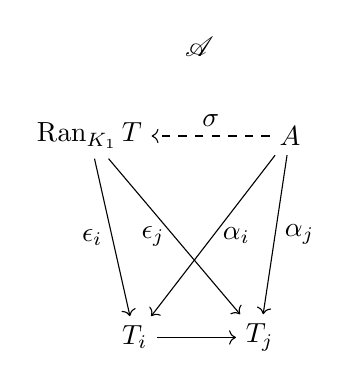
\begin{tikzpicture}
      \node (catA) {$\cat{A}$};
      \node [below left=0.6cm and 0.3cm of catA] (ran) {$\ran_{K_1}T$};
      \node [below right=2.0cm and -0.5cm of ran] (Ti) {$T_i$};
      \node [right=1.0cm of Ti] (Tj) {$T_j$};
      \draw [->] (Ti) to node [above] {} (Tj);
      \draw [->] (ran) to node [left] {$\epsilon_i$} (Ti);
      \draw [->] (ran) to node [left] {$\epsilon_j$} (Tj);
      \node [right=1.5cm of ran] (A) {$A$};
      \draw [->,dashed] (A) to node [above] {$\sigma$} (ran);
      \draw [->] (A) to node [right] {$\alpha_i$} (Ti);
      \draw [->] (A) to node [right] {$\alpha_j$} (Tj);
    \end{tikzpicture}
  \end{minipage}
\end{center}

\begin{theorem}[余極限は左カン拡張である\cite{maclane:kan-extensions}]
  函手 $T:\cat{M}\to\cat{A}$ について以下の2つは同値である:
  \begin{itemize}
    \item $T$ が余極限をもつ,
    \item $T$ が (一意的な) 函手 $K_1:\cat{M}\to\mathbf{1}$
          に沿った左カン拡張をもつ.
  \end{itemize}
  またこれらが成り立つとき $\colim T\simeq\lan_{K_1}T$.
\end{theorem}

\begin{proof}
  \cref{thm:limit-is-right-kan-extension} より双対的に示される.
\end{proof}

\begin{center}
  \begin{minipage}[b]{0.4\linewidth}
    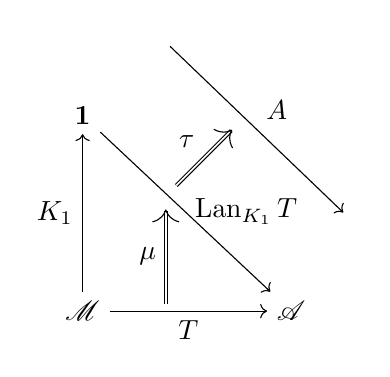
\begin{tikzpicture}
      \node (1) {$\mathbf{1}$};
      \node [below=2cm of 1] (M) {$\cat{M}$};
      \node [right=2cm of M] (A) {$\cat{A}$};
      \draw [->] (M) to node [left]         {$K_1$}      (1);
      \draw [->] (M) to node [below]        {$T$}        (A);
      \draw [->] (1) to node [right]  {$\lan_{K_1}T$} (A);
      \node [above right=0.9cm of 1] (astart) {};
      \node [below right=2.1cm and 2.2cm of astart] (aend) {};
      \draw [->] (astart) to node [above right] {$A$} (aend);
      \node [below right=1cm of 1] (estart) {};
      \node [below=1.2cm of estart] (eend) {};
      \draw [->,double] (eend) to node [left] {$\mu$} (estart);
      \node [above right=1.1cm and 0.6cm of M] (send) {};
      \node [above right=1.0cm of send] (sstart) {};
      \draw [->,double] (send) to node [above left] {$\tau$} (sstart);
    \end{tikzpicture}
  \end{minipage}
  \begin{minipage}[b]{0.4\linewidth}
    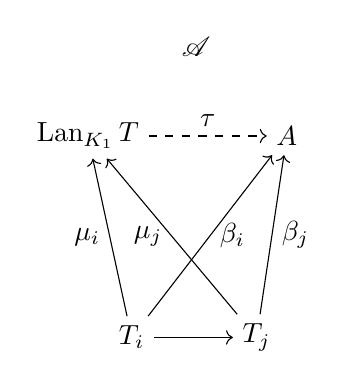
\begin{tikzpicture}
      \node (catA) {$\cat{A}$};
      \node [below left=0.6cm and 0.3cm of catA] (ran) {$\lan_{K_1}T$};
      \node [below right=2.0cm and -0.5cm of ran] (Ti) {$T_i$};
      \node [right=1.0cm of Ti] (Tj) {$T_j$};
      \draw [->] (Ti) to node [above] {} (Tj);
      \draw [->] (Ti) to node [left] {$\mu_i$} (ran);
      \draw [->] (Tj) to node [left] {$\mu_j$} (ran);
      \node [right=1.5cm of ran] (A) {$A$};
      \draw [->,dashed] (ran) to node [above] {$\tau$} (A);
      \draw [->] (Ti) to node [right] {$\beta_i$} (A);
      \draw [->] (Tj) to node [right] {$\beta_j$} (A);
    \end{tikzpicture}
  \end{minipage}
\end{center}

\chapter{圏論の応用}

\section{ストーンの双対性定理}

ストーンの双対性定理は,
(sober 性を満たす)
位相空間と
(空間的)
完備ハイティング代数が一対一に対応することを示す.
ふつう位相空間論は集合論の土台の上で定式化されるが,
この定理によって集合論ではなく束論に基づく位相空間論の定式化
(ポイントレス位相空間論)
が可能になる.

\subsection{ストーンの表現定理}

ストーンの表現定理は双対性定理の特別な場合である.
ストーンの双対性定理は位相空間と束の対応を与えるが,
ストーンの表現定理はそれらに制約を加えたストーン空間とブール代数の対応を与える.

\begin{definition}[ストーン空間の圏]
  ストーン空間
  (\cref{def:stone-space})
  と連続写像
  (\cref{def:continuous-map})
  のなす圏を $\stone$ と表記する.
\end{definition}

\begin{definition}[ブール代数の圏]
  ブール代数 (\cref{def:boolean-algebra})
  とブール準同型のなす圏を $\blat$ と表記する.
\end{definition}

\newcommand{\spec}{\operatorname{spec}}
\newcommand{\clop}{\operatorname{clop}}

\begin{theorem}[ストーンの表現定理]
  \begin{equation}
    \stone\simeq\blat^\mathrm{op}.
  \end{equation}
\end{theorem}

\begin{proof}
  反変函手 $\spec:\blat^\mathrm{op}\to\stone$ および
  $\clop:\stone^\mathrm{op}\to\blat$ を定め,自然同型
  $\eta:\id{\blat}\simeq\clop\circ(\spec^\mathrm{op})$ が存在することを示す.
  以下,メモ.
  \begin{itemize}
    \item $\spec(B)$: ブール準同型 $B\to2$ の全体
          \begin{itemize}
            \item 集合 $2$ に離散位相を入れて $2^B$ に積位相を入れた位相空間を
                  考えると,$\spec(B)\subseteq 2^B$ はその部分位相空間になる
          \end{itemize}
    \item $\spec(b:B'\to B)=b^{-1}:\spec(B)\to\spec(B')$
          \begin{itemize}
            \item $b^{-1}$ は $b$ の逆像を与える
          \end{itemize}
    \item 反変函手 $\clop:\stone^\mathrm{op}\to\blat$
          \begin{itemize}
            \item $\clop(X)$: $X$ の開かつ閉集合の全体
            \item 和集合および積集合を取る操作について閉じており,ブール代数となる
          \end{itemize}
    \item $\eta_B:B\ni b\mapsto\{v\in\spec(B)\mid v(b)=1\}\in\clop(\spec(B))$
  \end{itemize}
\end{proof}

\subsection{ストーンの双対性定理}

\begin{definition}[既約]
  以下の条件を満たす位相空間
  $(X,\mathcal{O})$
  を既約
  (irreducible)
  であるという.
  \begin{equation}
    \forall O_1,O_2\in\mathcal{O}\setminus\{\emptyset\};
    \ (X\setminus O_1)\cap(X\setminus O_2)\neq X
  \end{equation}
\end{definition}

\begin{definition}[sober 空間]
  既約位相空間
  $(X,\mathcal{O})$
  の任意の既約閉部分集合
  $A\subseteq X$
  について,
  $\{a\}$
  の閉包が
  $A$
  に等しくなるような
  $a\in A$
  がただ一つ存在するとき,
  $(X,\mathcal{O})$
  を sober 空間 (sober space) という.
\end{definition}

\begin{definition}[空間的完備ハイティング代数]
  完備
  (\cref{def:complete-lattice})
  なハイティング代数
  (\cref{def:heyting-algebra})
  $F$
  について,任意の
  $a,b\in F$
  に対して
  $a\le b$
  でないならば
  $f(a)=1\wedge f(b)=0$
  を満たす束準同型
  $f:F\to\{0,1\}$
  が存在するとき,
  $F$
  を空間的完備ハイティング代数
  (spatial complete Heyting algebra)
  という。
\end{definition}

\newcommand{\sob}{\mathbf{Sob}}
\newcommand{\sfrm}{\mathbf{SFrm}}

\begin{definition}[sober 空間の圏]
  sober 空間と連続写像のなす圏を $\sob$ と表記する.
\end{definition}

\begin{definition}[空間的完備ハイティング代数の圏]
  空間的完備ハイティング代数と束準同型のなす圏を $\sfrm$ と表記する.
\end{definition}

\begin{theorem}[ストーンの双対性定理]
  \begin{equation}
    \sob\simeq\sfrm^\mathrm{op}.
  \end{equation}
\end{theorem}

{

\chapter{豊穣圏}

豊穣圏は,ここまで用いてきた普通の圏の概念の抽象化である.
本章以降では前章までの定義や表記を一切用いず,
全ての概念をより一般的に再定義する.

\section{豊穣圏}

\def\C{\cat{C}}%
\def\mcat{\cat{V}}%
\newcommand\tprod{\otimes}%
\newcommand\tunit{1}%
\newcommand\assoc{\alpha}%
\newcommand\lunit{\lambda}%
\newcommand\runit{\rho}%
\def\a{\obj{a}}%
\def\b{\obj{b}}%
\def\c{\obj{c}}%
\def\d{\obj{d}}%

普通の圏においては,
任意の対象のペアの間に射の集合 (または集まり) が与えられていた.
豊穣圏では,その「射の集合」はモノイド圏の対象として与えられる.

\begin{definition}[豊穣圏]
  モノイド圏 (\cref{def:monoidal-category})
  $(\mcat,\tprod,\tunit,\assoc,\lunit,\runit)$ について,
  $\mcat$-豊穣圏 ($\mcat$-enriched category) $\C$ は以下の条件を満たす:
  \begin{itemize}
    \item 対象の集まりをもつ.
    \item 任意の対象 $\a,\b\in\objs{\C}$ に対して
          $\mrps{\C}{\a}{\b}\in\mcat$ が存在する.
    \item 任意の対象 $\a,\b,\c\in\objs{\C}$ に対して $\mcat$ の射
          \begin{equation}
            \mrp{{m}_{\a,\b,\c}}{
              \mrps{\C}{\b}{\c}\tprod\mrps{\C}{\a}{\b}
            }{\mrps{\C}{\a}{\c}}
          \end{equation}
          が存在し,
          任意の対象 $\a,\b,\c\in\objs{\C}$ に対して以下の図式を可換にする:
          \begin{center}
            \begin{tikzcd}
              (\mrps{\C}{\c}{\d}\tprod\mrps{\C}{\b}{\c})\tprod\mrps{\C}{\a}{\b}
              \arrow{rr}{
                \assoc_{\mrps{\C}{\c}{\d},\mrps{\C}{\b}{\c},\mrps{\C}{\a}{\b}}
              }
              \arrow{d}[swap]{m_{\b,\c,\d}\tprod\id{\mrps{\C}{\a}{\b}}}
              &&
              \mrps{\C}{\c}{\d}\tprod(\mrps{\C}{\b}{\c}\tprod\mrps{\C}{\a}{\b})
              \arrow{d}{\id{\mrps{\C}{\c}{\d}}\tprod{m}_{\a,\b,\c}} \\
              \mrps{\C}{\b}{\d}\tprod\mrps{\C}{\a}{\b}
              \arrow{r}[swap]{m_{\a,\b,\d}}
              & \mrps{\C}{\a}{\d}
              & \mrps{\C}{\c}{\d}\tprod\mrps{\C}{\a}{\c}
              \arrow{l}{m_{\a,\c,\d}}
            \end{tikzcd}
          \end{center}
    \item 任意の対象 $\a\in\objs{\C}$ に対して $\mcat$ の射
          \begin{equation}
            \mrp{{j}_{\a}}{\tunit}{\mrps{\C}{\a}{\a}}
          \end{equation}
          が存在し,
          任意の対象 $\a,\b\in\objs{\C}$ に対して以下の図式を可換にする:
          \begin{center}
            \begin{tikzcd}
              \tunit\tprod\mrps{\C}{\a}{\b}
              \arrow{r}{\lunit_{\mrps{\C}{\a}{\b}}}
              \arrow{d}[swap]{j_{\b}\tprod\id{\mrps{\C}{\a}{\b}}}
              & \mrps{\C}{\a}{\b}
              & \mrps{\C}{\a}{\b}\tprod\tunit%
              \arrow{l}[swap]{\runit_{\mrps{\C}{\a}{\b}}}
              \arrow{d}{\id{\mrps{\C}{\a}{\b}}\tprod{j_{\a}}} \\
              \mrps{\C}{\b}{\b}\tprod\mrps{\C}{\a}{\b}
              \arrow{ru}[swap]{m_{\a,\b,\b}}
              && \mrps{\C}{\a}{\b}\tprod\mrps{\C}{\a}{\a}
              \arrow{lu}{m_{\a,\a,\b}}
            \end{tikzcd}
          \end{center}
  \end{itemize}
\end{definition}

}

\bibliography{main}
\bibliographystyle{unsrt}

\appendix

\chapter{基礎論}

\begin{definition}[グロタンディーク宇宙]
  \def\U{U}%
  \def\x{x}%
  \def\y{y}%
  以下の性質をもつ集合 $\U$ を
  グロタンディーク宇宙 (Grothendieck universe) という.
  \begin{align}
     & \forall\x\in\U\ \forall\y\in\x;\ \x\in\U,              \\
     & \forall\x,\y\in\U;\ \{\x,\y\}\in\U,                    \\
     & \forall\x\in\U;\ 2^\x\in\U,                            \\
     & \forall I\in\U\ \forall{\{\x_i\}}_{i\in I}\subseteq\U;
    \ \bigcup_{i\in I}\x_i\in\U.
  \end{align}
\end{definition}

\begin{definition}[小さい集合]\label{def:small-set}
  グロタンディーク宇宙の元を小さい集合 (small set) という.
\end{definition}

\chapter{代数学の知識}

 {

  \section{群論}

  \def\x{x}%
  \def\y{y}%
  \def\z{z}%
  \def\munit{1}%

  \begin{definition}[マグマ\cite{wiki:magma}]
    \def\magma{M}%
    集合 $\magma$ と二項演算 $\cdot:\magma\times\magma\to\magma$ の組
    $(\magma,\cdot)$ をマグマ (magma) という.
  \end{definition}

  \begin{definition}[半群\cite{wiki:semigroup}]
    \def\semigroup{S}%
    マグマ $(\semigroup,\cdot)$ が結合律
    \begin{equation}
      \forall\x,\y,\z\in\semigroup;\ (\x\cdot\y)\cdot\z=\x\cdot(\y\cdot\z)
    \end{equation}
    を満たすとき,$(\semigroup,\cdot)$ を半群 (semigroup) という.
  \end{definition}

  \begin{definition}[モノイド\cite{wiki:monoid}]
    \def\monoid{M}%
    半群 $(\monoid,\cdot)$ の元 $\munit\in\monoid$ が単位律
    \begin{equation}
      \forall\x\in\monoid;\ \munit\cdot\x=\x\cdot\munit=\x
    \end{equation}
    を満たすとき,$(\monoid,\cdot,\munit)$ をモノイド (monoid) という.
    また $\munit$ を単位元 (unit) という.
  \end{definition}

  \begin{definition}[群\cite{wiki:group}]
    \def\group{G}%
    モノイド $(\group,\cdot,\munit)$ の任意の元 $\x\in\group$ に対して
    $\x^{-1}\in\group$ が存在して
    \begin{equation}
      \x\cdot\x^{-1}=\x^{-1}\cdot\x=\munit
    \end{equation}
    が成り立つとき,$(\group,\cdot)$ を群 (group) という.
    また $\x^{-1}$ を $\x$ の逆元 (inverse) という.
  \end{definition}

  \begin{table}
    \centering
    \caption{代数的構造の階層}
    \begin{tabular}{cccc}
      \toprule
           & 結合律          & 単位元の存在       & 逆元の存在        \\
      \midrule
      マグマ  & {-}          & {-}          & {-}          \\
      半群   & \checkmark{} & {-}          & {-}          \\
      モノイド & \checkmark{} & \checkmark{} & {-}          \\
      群    & \checkmark{} & \checkmark{} & \checkmark{} \\
      \bottomrule
    \end{tabular}
  \end{table}
 }

\section{束論}

ハイティング代数は半順序,交わりと結び,最大元と最小元,
相対擬補元をそなえた代数構造であり,
ブール代数は相対擬補元が補元に一致するハイティング代数である.
普通これらの構造は集合論の土台の上で定義されるが,
圏論の概念を用いて定義することもできる.
例えば交わりと結びは積と余積として,最大元と最小限は終対象と始対象として,
相対擬補元は冪として表現することができる.

\begin{definition}[擬順序集合]
  \def\S{S}%
  \def\x{x}%
  \def\y{y}%
  \def\z{z}%
  集合 $S$ と二項関係 $\le$ が
  \begin{align}
    \forall\x\in\S       & ;\ \x\le\x,                           \\
    \forall\x,\y,\z\in\S & ;\ \x\le\y\land\y\le\z\implies\x\le\z
  \end{align}
  を満たすとき,$(\S,\le)$ を擬順序集合 (quasi-ordered set) または
  前順序集合 (preordered set) という.
\end{definition}

\begin{definition}[半順序集合]
  圏 $\cat{C}$ について
  \begin{equation}
    \forall x,y\in\objs{\cat{C}};|\mrps{\cat{C}}{x}{y}|\le1
  \end{equation}
  が成り立つとき,
  $\cat{C}$ は半順序集合 (partially ordered set, poset)
  であるという.
\end{definition}

\begin{definition}[束]
  半順序集合 $\cat{C}$ が
  有限積と有限余積をもつとき,
  $\cat{C}$ は束 (lattice) であるという.
\end{definition}

\begin{definition}[完備束]\label{def:complete-lattice}%
  任意の部分集合が下限と上限をもつような半順序集合を
  完備束
  (complete lattice)
  という.
\end{definition}

\begin{definition}[有界束]
  束 $\cat{C}$ が終対象と始対象をもつとき,
  $\cat{C}$ は有界束 (bounded lattice) であるという.
\end{definition}

\begin{definition}[ハイティング代数]\label{def:heyting-algebra}%
  有界束 $\cat{C}$ が任意の対象の組について冪をもつとき,
  $\cat{C}$ はハイティング代数 (Heyting algebra) であるという.
\end{definition}

\begin{theorem}
  任意の位相空間 (\cref{def:topological-space})
  の位相は完備ハイティング代数である.
\end{theorem}

\begin{definition}[ブール代数]\label{def:boolean-algebra}
  ハイティング代数 $\cat{C}$ について
  \begin{equation}
    \forall x\in\objs{\cat{C}};\ \neg\neg x=x
  \end{equation}
  が成り立つとき,
  $\cat{C}$ は ブール代数 (Boolean algebra) であるという.
\end{definition}

\chapter{位相幾何学の知識}

\section{位相空間論}

\begin{definition}[位相空間]\label{def:topological-space}
  集合 $X$ とその部分集合族 $\mathcal{O}\subseteq2^X$ が以下の条件を満たすとき,
  $(X,\mathcal{O})$ は位相空間 (topological space) であるといい,
  $\mathcal{O}$ を $X$ 上の位相 (topology) という.
  \begin{align}
    \emptyset,X\in\mathcal{O}                                 \\
    \forall O_1,O_2\in\mathcal{O};\ O_1\cup O_2\in\mathcal{O} \\
    \forall \mathcal{O}'\subseteq\mathcal{O};
    \bigcup_{O\in\mathcal{O}'}O\in\mathcal{O}
  \end{align}
\end{definition}

\begin{definition}[離散位相]
  位相空間 $(X,2^X)$ を離散位相空間 (discrete topological space) といい,
  $2^X$ を $X$ 上の離散位相 (discrete topology) という.
\end{definition}

\begin{definition}[密着位相]
  位相空間 $(X,\{\emptyset,X\})$
  を密着位相空間 (indiscrete topological space) といい,
  $\{\emptyset,X\}$ を $X$ 上の密着位相 (indiscrete topology)
  または自明な位相 (trivial topology) という.
\end{definition}

\begin{definition}[開集合,閉集合,開かつ閉集合]
  位相空間 $(X,\mathcal{O})$ について,
  $\mathcal{O}$ の元を $X$ の開集合 (open set) という.
  また部分集合 $S\subseteq X$ が
  \begin{equation}
    \exists O\in\mathcal{O};\ S=X\setminus O
  \end{equation}
  を満たすとき,
  $S$ は $X$ の閉集合 (closed set) であるという.

  $X$ の開集合でありかつ $X$ の閉集合である集合を
  $X$ の開かつ閉集合 (closed-open set, clopen set) という.
\end{definition}

\begin{definition}[連続写像]\label{def:continuous-map}
  位相空間 $(X,\mathcal{O}_X)$ と $(Y,\mathcal{O}_Y)$ および写像 $f:X\to Y$ が
  \begin{equation}
    \forall O\in\mathcal{O}_Y;\ f^{-1}(O)\in\mathcal{O}_X
  \end{equation}
  を満たすとき,
  $f$ は連続写像 (continuous map) であるという.
\end{definition}

\begin{definition}[被覆,開被覆,部分被覆,有限部分被覆]
  位相空間 $(X,\mathcal{O})$ の部分集合族 $\mathcal{C}\subseteq2^X$ について
  \begin{equation}
    X\subset\bigcup_{C\in\mathcal{C}}C
  \end{equation}
  が成り立つとき,
  $\mathcal{C}$ は $X$ の被覆 (cover) であるという.
  さらに $\mathcal{C}\subseteq\mathcal{O}$ であるとき,
  $\mathcal{C}$ は $X$ の開被覆 (open cover) であるという.

  また,
  $X$ の被覆 $\mathcal{C}_0\subseteq\mathcal{C}$ を
  $\mathcal{C}$ の部分被覆 (subcover) といい,
  さらに $\mathcal{C}_0$ が有限集合であるとき
  $\mathcal{C}_0$ は $\mathcal{C}$ の有限部分被覆 (finite subcover) であるという.
\end{definition}

\begin{definition}[コンパクト集合]
  位相空間 $(X,\mathcal{O})$ の部分集合 $A\subseteq X$ の
  任意の開被覆が有限部分被覆をもつとき,
  $A$ はコンパクト集合 (compact set) であるという.
\end{definition}

\begin{definition}[コンパクト空間]
  位相空間 $(X,\mathcal{O})$ について $X$ がコンパクト集合であるとき,
  $(X,\mathcal{O})$ はコンパクト空間 (compact space) であるという.
\end{definition}

\begin{example}[$\mathbb{R}$ はコンパクト空間でない]
  通常の位相をもつ
  $\mathbb{R}$
  の開被覆
  $\{(n,n+2)\mid n\in\mathbb{Z}\}$
  は有限部分被覆をもたないため,
  $\mathbb{R}$
  はコンパクト空間でない.
\end{example}

\begin{definition}[連結,不連結]
  位相空間 $(X,\mathcal{O})$ の部分集合 $A\subseteq X$ が
  \begin{equation}
    \exists O_1,O_2\in\mathcal{O}\setminus\{\emptyset\};
    \ O_1\cup O_2=A\wedge O_1\cap O_2=\emptyset
  \end{equation}
  を満たすとき $A$ は不連結 (disconnected) であるといい,
  不連結でない $X$ の部分集合は連結 (connected) であるという.
\end{definition}

\begin{definition}[連結成分]
  位相空間の極大な連結部分集合を,
  その位相空間の連結成分 (connected component) という.
\end{definition}

\begin{definition}[完全不連結]
  任意の連結成分が一点集合であるような位相空間を
  完全不連結 (disconnected) であるという.
\end{definition}

\begin{definition}[ハウスドルフ空間]
  以下の条件を満たす位相空間 $(X,\mathcal{O})$ を
  ハウスドルフ空間 (Hausdorff space) という.
  \begin{equation}
    \forall x,y\in X;
    \ \left[x\neq y\Longrightarrow\exists O_1,O_2\in\mathcal{O};
      \ x\in O_1\wedge y\in O_2\wedge O_1\cap O_2=\emptyset\right].
  \end{equation}
\end{definition}

\begin{definition}[ストーン空間]\label{def:stone-space}
  コンパクト完全不連結ハウスドルフ空間をストーン空間 (Stone space) という.
\end{definition}

\begin{theorem}[チコノフの定理]
  任意のコンパクト空間族の直積空間はコンパクト空間である.
\end{theorem}

\end{document}
